\newcommand{\lang}{english}

\ifdefined\ishandout
\newcommand{\handoutmode}{handout}
\else
\newcommand{\handoutmode}{}
\fi

\documentclass[10pt,
\lang ,
\handoutmode ,
compress
]{beamer}


\usepackage{ifthen}

\newcommand{\unibastring}{\ifthenelse{\equal{\lang}{ngerman}}{University of Bamberg}{University of Bamberg}}


\usepackage{eurosym}
\usepackage{etex}
\usepackage{ulem}
\usepackage{stmaryrd}
\usetheme{UniBa}
%\usefonttheme{
%	default | professionalfonts | serif |
%	structurebold | structureitalicserif |
%	structuresmallcapsserif
%}
\usefonttheme{professionalfonts}
%\useinnertheme{
%	circles | default | inmargin |
%	rectangles | rounded
%}
\useinnertheme{rectangles}
%\useoutertheme{
%	default | infolines | miniframes |
%	shadow | sidebar | smoothbars |
%	smoothtree | split | tree
%}
%\useoutertheme{split}
\setbeamercovered{transparent}

% Without navigation symbols
\beamertemplatenavigationsymbolsempty

%% Formatierungen
\usepackage{url}
\usepackage{latexsym}			% schönere Symbole
\usepackage{color}
%\usepackage{float}

%% Zeichensätze
\usepackage[utf8]{inputenc}
\usepackage{lmodern}
\usepackage{float}
%\usepackage{thumbpdf}
\usepackage{wasysym}
%\usepackage{ucs}

%Meta info
%Necessary Information
\author[Fachschaft WIAI, University of Bamberg]{Student Association\\Information Systems and Applied Computer Sciences}
\title{\LaTeX ~-Tutorial by Fachschaft WIAI}
%The day of the presentation
\date{\today}

%Optional Information
\subject{subject}
\keywords{keywords}

%Already set
\institute[This work is licensed under a Creative Commons Attribution-ShareAlike 4.0 International License]{Professorship for Computer Science,\\ Communication Services, Telecommunication Systems and Computer Networks}

\titlegraphic{
\includegraphics[height=20mm]{image/wiailogo}\hspace{2.2cm}\includegraphics[height=20pt]{image/by-sa.eps}\hspace{2.2cm}
\includegraphics[height=20mm]{image/logo}}


%% Hyperref
\usepackage{hyperref}

\makeatletter
\hypersetup{pdftitle={\@title}, pdfauthor={\@author}, linktoc=page, pdfborder={0 0 0 [3 3]}, breaklinks=true, linkbordercolor=unibablueI, menubordercolor=unibablueI, urlbordercolor=unibablueI, citebordercolor=unibablueI, filebordercolor=unibablueI}
\makeatother
%% Define a new 'leo' style for the package that will use a smaller font.
\makeatletter
\def\url@leostyle{%
  \@ifundefined{selectfont}{\def\UrlFont{\sf}}{\def\UrlFont{\small\ttfamily}}}
\makeatother
%% Now actually use the newly defined style.
\urlstyle{leo}

%% Sprache
\ifthenelse{\equal{\lang}{ngerman}}{\usepackage[german,ngerman]{babel}}{\usepackage[\lang]{babel}}
%\mode<presentation>{
%% XXX without this the number does not appear
%\AtBeginDocument{\def\figurename{{\scshape Fig.~\thefigure}}}
%}
%%\usepackage{abstract}

%% Mathe und Formeln
\usepackage{calc}
\usepackage{amsmath}
\usepackage{amssymb,amsthm,amsfonts}
\usepackage{dsfont}
\usepackage[nice]{nicefrac}
\usepackage{cancel}  %%druchstreichen von Formeln
%
%% Programmieren mit Latex
\usepackage{ifthen}


\usepackage{dirtree}   %setzen von baumstrukturen

%%%   Fuer anspruchsvolle Tabellen   %%
\usepackage{longtable, colortbl}
\usepackage{multicol, multirow}
%
%%%  Für Grafiken %%
\usepackage{graphicx}
\usepackage{tikz}
%\usepackage{pgfplots}
\usetikzlibrary{calc,arrows,fit,positioning,trees,backgrounds,shadows,decorations,decorations.markings,decorations.shapes,shapes,patterns,fadings}
\usepackage[font=footnotesize]{subfig}


\makeatletter
\newcount\dirtree@lvl
\newcount\dirtree@plvl
\newcount\dirtree@clvl
\def\dirtree@growth{%
  \ifnum\tikznumberofcurrentchild=1\relax
  \global\advance\dirtree@plvl by 1
  \expandafter\xdef\csname dirtree@p@\the\dirtree@plvl\endcsname{\the\dirtree@lvl}
  \fi
  \global\advance\dirtree@lvl by 1\relax
  \dirtree@clvl=\dirtree@lvl
  \advance\dirtree@clvl by -\csname dirtree@p@\the\dirtree@plvl\endcsname
  \pgf@xa=1cm\relax
  \pgf@ya=-1cm\relax
  \pgf@ya=\dirtree@clvl\pgf@ya
  \pgftransformshift{\pgfqpoint{\the\pgf@xa}{\the\pgf@ya}}%
  \ifnum\tikznumberofcurrentchild=\tikznumberofchildren
  \global\advance\dirtree@plvl by -1
  \fi
}

\tikzset{
  dirtree/.style={
    growth function=\dirtree@growth,
    every node/.style={anchor=north},
    every child node/.style={anchor=west},
    edge from parent path={(\tikzparentnode\tikzparentanchor) |- (\tikzchildnode\tikzchildanchor)}
  }
}
\makeatother
%\usepackage{fp}
%
%%%  Zur Darstellung des Euro-Symbols   %%
%\usepackage{eurosym, wasysym}
%\selectlanguage{german}
%
%%%   Fuer Bibtex nach APA Style (American Psychology Association)   %%
%\usepackage[numbers]{natbib}
\usebibitemtemplate{\insertbiblabel}

%% Code-Hervorhebung
%% Quellcode

%\usepackage[numbered,autolinebreaks,useliterate]{mcode}
%\usepackage{verbatim}            % Quellcode einbinden (\verbatiminput) standardpaket
%\usepackage{moreverb} 
%% PseudoCode
%\usepackage{algorithm}
\usepackage{algpseudocode}
%%\usepackage{algorithmicx}
%%\floatname{algorithm}{Algorithmus}
%\algrenewcommand{\algorithmiccomment}[1]{\hskip1em\textcolor{gray!60}{$\rhd$ #1}}
%%\renewcommand{\listalgorithmname}{Algorithmen}
%%\def\algorithmautorefname{Algorithmus}
%
%%% Code Highlighting
%\definecolor{mygray}{gray}{.75}
%\usepackage{listings} 
%\lstset{numbers=left, numberstyle=\tiny, numbersep=6pt} 
%\lstset{language=Python}
%\lstset{classoffset=1, morekeywords={mycontext}, keywordstyle=\color{darkgreen}, classoffset=0, keywordstyle=\color{darkblue}}
%\lstset{basicstyle=\small, showstringspaces=false, commentstyle=\color{mygray}, breaklines=true, captionpos=b}
%\renewcommand{\lstlistingname}{Code-Ausschnitt}
%\renewcommand{\lstlistlistingname}{Code-Ausschnitte}
%\def\lstlistingautorefname{Code-Ausschnitt}


%%%%%%%%%%%%%%%%%%%%%%%%%%%%%%%%%%%%%%%%%%%%%%%%%%%%%%%%%%%%%%%%%%%%%%%%%%%%%%%%%%%%%%%%%%%%
%%%                                   COMMAND SETUP                                       %%
%%%%%%%%%%%%%%%%%%%%%%%%%%%%%%%%%%%%%%%%%%%%%%%%%%%%%%%%%%%%%%%%%%%%%%%%%%%%%%%%%%%%%%%%%%%%

%#1 Breite
%#2 Datei (liegt im image Verzeichnis)
%#3 Beschriftung
%#4 Label fuer Referenzierung
\newcommand{\image}[4]{
\begin{figure}[H]
\centering
\includegraphics[width=#1]{#2}
\caption{\footnotesize{#3}}
\label{#4}
\end{figure}
}

% #1 videofile
% #2 scalefactor
\newcommand{\video}[2]{%
\includemovie[text={\includegraphics[scale=#2]{praesi/video/#1.png}}, autoplay, mouse=true, repeat=1]{}{}{praesi/video/#1.swf}}


\def\signed #1{{\leavevmode\unskip\nobreak\hfil\penalty50\hskip2em
  \hbox{}\nobreak\hfil(#1)%
  \parfillskip=0pt \finalhyphendemerits=0 \endgraf}}

\newsavebox\mybox
\newenvironment{aquote}[1]
  {\savebox\mybox{#1}\begin{fancyquotes}}
  {\signed{\usebox\mybox}\end{fancyquotes}}


\hyphenation{op-tical net-works semi-conduc-tor}

\setbeamertemplate{caption}[numbered]
%\numberwithin{figure}{section}
\begin{document}

\frame{\titlepage}

\AtBeginSection[]
{
  \frame<handout:0>
  {
    \frametitle{Outline}
    \begin{multicols}{2}
    \tableofcontents[currentsection,hideallsubsections]
    \end{multicols}
  }
}

%\AtBeginSubsection[]
%{
%  \frame<handout:0>
%  {
%    \frametitle{Outline}
%    \tableofcontents[sectionstyle=show/hide,subsectionstyle=show/shaded/hide,subsubsectionstyle=hide]
%  }
%}

%\AtBeginSubsubsection[]
%{
%  \frame<handout:0>
%  {
%    \frametitle{Outline}
%    \tableofcontents[sectionstyle=show/hide,subsectionstyle=show/shaded/hide,subsubsectionstyle=show/shaded/hide]
%  }
%}

\newcommand<>{\highlighton}[1]{%
  \alt#2{\structure{#1}}{{#1}}
}

\newcommand{\icon}[1]{\pgfimage[height=1em]{#1}}

\begin{frame}
\frametitle{About this tutorial}
%\begin{block}{"Uber dieses Tutorium}
\begin{itemize}
\item Powered by Prof.\,Dr.\,Udo Krieger
\item Version 9.2
\item Changed to \LaTeX -Beamer and extended by Linus Dietz
\item English Version by Valentin Barth
\item Original slide set by\begin{itemize}
\item Marcel Grossmann
\item Steffen Illig
\item Martin Sticht
\item Michael Timpelan
\end{itemize}
\item ca. 2500 LOC (Lines of Code)
\end{itemize}
%\end{block}
\end{frame}

\begin{frame}{\contentsname}
    \frametitle{Outline}
\begin{multicols}{2}
\tableofcontents[hideallsubsections]
\end{multicols}
\end{frame}


%%%%%%%%%%%%%%%%%%%%%%%%%%%%%%%%%%%%%%%%%
%%%%%%%%%% Content starts here %%%%%%%%%%
%%%%%%%%%%%%%%%%%%%%%%%%%%%%%%%%%%%%%%%%%
%\input{content/spielwiese}
\section{Intro} 

\subsection{Scope, Sense and Purpose}
\begin{frame}[t]
\frametitle{Introduction}
\framesubtitle{Sense -- Nonsense -- Madness}
\bigskip
\bigskip
\bigskip

\begin{columns}[t]
\begin{column}{.3\textwidth}
\textbf{Useful}\\[3mm]
\begin{itemize}
\item Articles
\item Books
\item Scientific papers
\item Applications
\end{itemize}
\end{column}
\begin{column}{.30\textwidth}
\textbf{Nonsense}\\[3mm]
\begin{itemize}
\item Private mail
\item Invitations to your birthday party
\item Drink Menu
\end{itemize}
\end{column}
\begin{column}{.3\textwidth}
\textbf{Madness}\\[3mm]
\begin{itemize}
\item Shopping list
\item Brainstorming
\item \ldots 
\end{itemize}
\end{column}
\end{columns}
\end{frame}

%-------------------------------------------------------------------------------

\begin{frame} 
\frametitle{From Code To Document}
\framesubtitle{No WYSIWYG} 
\begin{columns}
\begin{column}{.7\textwidth}
\image{\textwidth}{image/worddoc.jpg}{\textbf{W}hat \textbf{Y}ou \textbf{S}ee \textbf{I}s \textbf{W}hat \textbf{Y}ou
\textbf{G}et}{img:worddoc}
\end{column}
\begin{column}{.3\textwidth}
\image{\textwidth}{image/codescreen.png}{\textbf{W}hat \textbf{W}ill \textbf{I} \textbf{G}et?}{img:codescreen}
%% Compile Animation
\end{column}
\end{columns}
\end{frame}

%-------------------------------------------------------------------------------

\begin{frame}
\frametitle{Introduction}
\framesubtitle{Approach}
\begin{columns}[onlytextwidth]
\begin{column}{0.40\textwidth}
\image{.8\textwidth}{image/codescreen.png}{Text File with \LaTeX ~-Code}{img:code}
\end{column}
\begin{column}{0.25\textwidth}
\image{.8\textwidth}{image/miktex.jpg}{Compiler (z.B. MikTeX)}{img:miktex}
\end{column}
\begin{column}{0.25\textwidth}
\image{.6\textwidth}{image/pdflogo.png}{good-looking, legible and printable document}{img:pdf}
\end{column}
\end{columns}
\end{frame}


%-------------------------------------------------------------------------------

\subsection{Advantages \& Disadvantages}
\begin{frame}
\frametitle{Introduction}
\framesubtitle{Advantages \& Disadvantages}
Advantages
\begin{itemize}
\item  dynamic directories and references
\item  automated layouts
\item  simple distributed work
\end{itemize}
Disadvantages
\begin{itemize}
\item  What do I get in the end?
\item  many, partly complex commands
\end{itemize}
\end{frame}

%-------------------------------------------------------------------------------

\subsection{\LaTeX --Compiler}
\begin{frame}
\frametitle{Introduction}
\framesubtitle{\LaTeX - Compiler}
\begin{columns}[t]
\begin{column}{.4\textwidth}
\textbf{Software for Windows:}\\
\begin{itemize}
  \item MikTex (http://www.miktex.org)\\
   2 alternatives: Basic or  Complete
  \item ProTeXt (http://www.tug.org/protext)\\
contains MikTex, TeXnicCenter and Ghostscript – simple installation\\
\end{itemize}
\end{column}
\begin{column}{.6\textwidth}
\textbf{Software for *nix:}
\begin{itemize}
  \item TeXLive\\
Packages for Ubuntu: {\ttfamily texlive-full} is the full meta-package with all necessary packages. Also contains the following:
\begin{itemize}
  \item {\ttfamily texlive-base
  \item texlive-lang-german}
\end{itemize}
Installation: {\ttfamily sudo apt-get install texlive-full}
\item MacOS: MacTeX (http://www.tug.org/mactex/2009)\\
\end{itemize}
\end{column}
\end{columns}
\end{frame}

%-------------------------------------------------------------------------------

\subsection{Free Editors}

\subsubsection{*nix}
\begin{frame}
\frametitle{Introduction}
\framesubtitle{Free Editors -- Linus \& MacOS }
\begin{itemize}
 \item Kile\footnote{http://kile.sourceforge.net/}\\KDE-program, also usable under Gnome\slash Unity etc.
 Installation for Debian systemes with {\ttfamily sudo apt-get
 install kile}.
  \item Vim \LaTeX -suite (Plugin)\footnote{http://vim-latex.sourceforge.net/}\\
  Dream for Vim users.
  \item TexShop (MacOS)\footnote{http://pages.uoregon.edu/koch/texshop/}
\end{itemize}
\end{frame}

%-------------------------------------------------------------------------------

\subsubsection{Windows}
\begin{frame}
\frametitle{Introduction}
\framesubtitle{Free Editors -- Windows}
\begin{itemize}
\item TeXnicCenter\footnote{http://www.texniccenter.org/}
  %\item \ldots
\end{itemize}
\end{frame}

%-------------------------------------------------------------------------------

\subsubsection{Cross-Platform}
\begin{frame}
\frametitle{Introduction}
\framesubtitle{Free Editors -- Cross-Platform}
\begin{itemize}
  \item TeXMaker\footnote{http://www.xm1math.net/texmaker}\\
   Used in this turorial.
  \item TeXstudio\footnote{http://sourceforge.net/projects/texstudio/?source=dlp}\\
  Like TeXMaker, but more powerful.
  \item TeXlipse\footnote{http://texlipse.sourceforge.net/}\\ For advanced users, plugin for
  Eclipse. Good IDE support, code-completion, autobuilds, version control etc.
\end{itemize}
\end{frame}

%-------------------------------------------------------------------------------

\begin{frame}
\frametitle{TeXmaker}
\framesubtitle{Overview}
\image{\textwidth}{image/texmaker_overview.png}{Standard window of the Texmaker}{img:texmaker1}

\end{frame}

%-------------------------------------------------------------------------------

\begin{frame}
\frametitle{TeXmaker}
\framesubtitle{Synctex}
\image{\textwidth}{image/synctex.png}{Synctex}{img:synctex}

\end{frame}

\begin{frame}
\frametitle{My very first \LaTeX -document}
\begin{block}{New commands:}
\begin{itemize}
\item \begin{ttfamily}\color{nounibaredII}\textbackslash documentclass\color{nounibagreenI}\color{black}\{article\}\end{ttfamily}
\item \begin{ttfamily}\color{unibablueI}\textbackslash begin\color{black}\{document\}\end{ttfamily}
\item \begin{ttfamily}\color{unibablueI}\textbackslash end\color{black}\{document\}\end{ttfamily}
\end{itemize}
\end{block}
This is all you need for a \LaTeX -document. Let's try!

\end{frame}

\section{$\mathcal{T}1$} 
\begin{frame}
\frametitle{Task 1}
\framesubtitle{Write and compile ``Hello World!''}
\begin{center}
\begin{rm}
\Large Hello World!\\
\end{rm}
\end{center}
\bigskip
\bigskip
\bigskip
\begin{block}{Task 1}
\begin{itemize}
\item Standard \LaTeX -files have the file extension {\ttfamily .tex}
\end{itemize}
\end{block}
\begin{alertblock}{\textbf{Attention:}}
Before you start, please create a new folder to save all your files in!
\end{alertblock}
\end{frame}

\section{Formatting}

\begin{frame}
\frametitle{A First Application Example}
\framesubtitle{Headlines, Table of Contents, simple formatting,
special characters}
\begin{block}{New commands in this section}
\begin{multicols}{2}
\begin{itemize}
  \item \begin{ttfamily}\color{nounibaredII}\textbackslash usepackage\color{black}\{package\}
  \item \color{nounibaredII}\textbackslash command\color{nounibagreenI}[poss\_options]\color{black}\{\\formatted\_text\}
  \item \color{unibablueI}\textbackslash begin\color{black}\{environment\}
  \item \color{unibablueI}\textbackslash end\color{black}\{environment\}
  \item \color{nounibaredII}$\backslash\backslash$\color{black}
  \item \color{nounibaredI}\textbackslash newpage\color{black}
  \item \color{unibablueI}\textbackslash sub$^*$section\color{black}\{Title\}
  \item $\color{nounibaredII}\backslash$\color{nounibaredII}textbf\color{black}\{Text\}
  \item $\color{nounibaredII}\backslash$\color{nounibaredII}textit\color{black}\{Text\}
  \item $\color{nounibaredII}\backslash$\color{nounibaredII}underline\color{black}\{Text\}
  \item \color{nounibaredI}$\color{nounibaredI}\backslash$tiny
  \item \color{nounibaredI}$\color{nounibaredI}\backslash$scriptsize
  \item \color{nounibaredI}$\color{nounibaredI}\backslash$footnotesize
  \item \color{nounibaredI}$\color{nounibaredI}\backslash$normalsize
  \item \color{nounibaredI}$\color{nounibaredI}\backslash$large
  \item \color{nounibaredI}$\color{nounibaredI}\backslash$Large
  \item \color{nounibaredI}$\color{nounibaredI}\backslash$LARGE
  \item \color{nounibaredI}$\color{nounibaredI}\backslash$huge\end{ttfamily}
\end{itemize}
\end{multicols}
\end{block}
\end{frame}


%\begin{frame}
%\frametitle{Ein erstes Anwendungsbeispiel}
%\framesubtitle{Pakete einbinden und Befehle anwenden}
%\begin{itemize}
%  \item Pakete sind Sammlungen von Befehlen oder enthalten z.B. Zeichensätze.\\ Sie werden zu
%  Beginn einer \TeX-Datei angegeben:\\
%  \smallskip
%\textbf{\begin{ttfamily}\color{nounibaredII}\textbackslash usepackage\color{black}\{babel\}
%
%\smallskip
%\end{ttfamily}}
% Einbinden des Paketes „\begin{ttfamily}babel\end{ttfamily}“. (F\"ur Internationalisierung)
%\item Schreibweise von Latex-Befehlen:
%
%\textbf{\begin{ttfamily}\color{nounibaredII}\textbackslash befehl\color{nounibagreenI}[evtl\_optionen]\color{black}\{Formatierter\_Text\}\end{ttfamily}}
%\begin{itemize}
%  \item in \begin{ttfamily}\{\}\end{ttfamily} stehen immer notwendige Parameter bzw. Text
% \item in \begin{ttfamily}[ ]\end{ttfamily} stehen (falls vorhanden)
% zus"atzliche, optionale Parameter
% \item zum Beispiel:
%
%
%\begin{ttfamily}
%\color{nounibaredII}\textbackslash documentclass\color{nounibagreenI}[a4paper,12pt,pdftex,ngerman]\color{black}\{article\}
%\end{ttfamily}
%\end{itemize}
%\end{frame}

\begin{frame}
\frametitle{A First Application Example}
\framesubtitle{Commands cont'd}
\begin{columns}
\begin{column}{0.6\textwidth}
\begin{ttfamily}\scriptsize
\color{nounibaredI}\color{nounibaredI}\textbackslash documentclass\color{black}\color{nounibagreenI}[a4paper, pdftex, ngerman]\color{black}\{article\} \\
\color{nounibaredI}\color{nounibaredI}\textbackslash usepackage\color{black}\color{nounibagreenI}[utf8]\color{black}\{inputenc\} \\
\color{nounibaredI}\color{nounibaredI}\textbackslash usepackage\color{black}\color{nounibagreenI}[T1]\color{black}\{fontenc\} \\
\color{nounibaredI}\color{unibablueI}\textbackslash\color{unibablueI}begin\color{black}\color{black}\{document\} \\
This is a simple document \\
without specials. Line breaks \\
are made automatically! \\
Multiple \\
consecutively blank characters  \\
are condensed to one. \\
Automatic hyphenation.\color{nounibaredI}\color{nounibaredI}\textbackslash \color{nounibaredI}\textbackslash \color{black} \\
Two backslashes make a line \\
break.\color{nounibaredI}\color{nounibaredI}\textbackslash \color{nounibaredI}\textbackslash \color{black} \\
A new paragraph is made by an\\
empty line.\\
\color{nounibaredI}\color{unibablueI}\textbackslash\color{unibablueI}end\color{black}\color{black}\{document\} \\

\end{ttfamily}
\end{column}

\begin{column}{0.4\textwidth}
There are different types of documents.\\ The document type
\begin{ttfamily}article\end{ttfamily} is used here (also possible:
\begin{ttfamily}book\end{ttfamily} and \begin{ttfamily}report\end{ttfamily}). The input in
\begin{ttfamily}[]\end{ttfamily} indicates paper size and font size of the
standard text.\\
%! TODO!
\end{column}
\end{columns}
\end{frame}

\begin{frame}
\frametitle{A First Application Example}
\framesubtitle{Commands cont'd}
\begin{columns}
\begin{column}{0.6\textwidth}
\begin{ttfamily}\scriptsize
\color{nounibaredI}\color{nounibaredI}\textbackslash documentclass\color{black}\color{nounibagreenI}[a4paper, pdftex, ngerman]\color{black}\{article\} \\
\color{nounibaredI}\color{nounibaredI}\textbackslash usepackage\color{black}\color{nounibagreenI}[utf8]\color{black}\{inputenc\} \\
\color{nounibaredI}\color{nounibaredI}\textbackslash usepackage\color{black}\color{nounibagreenI}[T1]\color{black}\{fontenc\} \\
\color{nounibaredI}\color{unibablueI}\textbackslash\color{unibablueI}begin\color{black}\color{black}\{document\} \\
This is a simple document \\
without specials. Line breaks \\
are made automatically! \\
Multiple \\
consecutively blank characters  \\
are condensed to one. \\
Automatic hyphenation.\color{nounibaredI}\color{nounibaredI}\textbackslash \color{nounibaredI}\textbackslash \color{black} \\
Two backslashes make a line \\
break.\color{nounibaredI}\color{nounibaredI}\textbackslash \color{nounibaredI}\textbackslash \color{black} \\
A new paragraph is made by an\\
empty line.\\
\color{nounibaredI}\color{unibablueI}\textbackslash\color{unibablueI}end\color{black}\color{black}\{document\} \\

 \normalsize
\end{ttfamily}
\end{column}
\begin{column}{0.4\textwidth}
\begin{ttfamily}\textbf{\color{unibablueI}\textbackslash begin\color{black}\{environment\}}\end{ttfamily}\\
A new environment begins, in this case the actual document.\\[5mm]

\begin{ttfamily}\textbf{\color{unibablueI}\textbackslash end\color{black}\{environment\}}\end{ttfamily}\\
The environment that started with \begin{ttfamily}\textbf{\color{unibablueI}\textbackslash begin}\color{black}\{\}\end{ttfamily}
ends here.\\[5mm]

\begin{ttfamily}\textbf{\color{nounibaredII}$\backslash\backslash$}\color{black}
~line break\end{ttfamily}\\
\end{column}
\end{columns}
\end{frame}



\begin{frame}
\frametitle{A First Application Example}
\framesubtitle{Packages}
\begin{columns}
\begin{column}{0.6\textwidth}
\begin{ttfamily}\scriptsize
\color{nounibaredI}\color{nounibaredI}\textbackslash documentclass\color{black}\color{nounibagreenI}[a4paper, pdftex, ngerman]\color{black}\{article\} \\
\color{nounibaredI}\color{nounibaredI}\textbackslash usepackage\color{black}\color{nounibagreenI}[utf8]\color{black}\{inputenc\} \\
\color{nounibaredI}\color{nounibaredI}\textbackslash usepackage\color{black}\color{nounibagreenI}[T1]\color{black}\{fontenc\} \\
\color{nounibaredI}\color{unibablueI}\textbackslash\color{unibablueI}begin\color{black}\color{black}\{document\} \\
This is a simple document \\
without specials. Line breaks \\
are made automatically! \\
Multiple \\
consecutively blank characters  \\
are condensed to one. \\
Automatic hyphenation.\color{nounibaredI}\color{nounibaredI}\textbackslash \color{nounibaredI}\textbackslash \color{black} \\
Two backslashes make a line \\
break.\color{nounibaredI}\color{nounibaredI}\textbackslash \color{nounibaredI}\textbackslash \color{black} \\
A new paragraph is made by an\\
empty line.\\
\color{nounibaredI}\color{unibablueI}\textbackslash\color{unibablueI}end\color{black}\color{black}\{document\} \\

 \normalsize
\end{ttfamily}
\end{column}
\begin{column}{0.4\textwidth}
\begin{ttfamily}\textbf{ngerman}\end{ttfamily}\\
The typical formattings and rules of the german language are used (instead of \grqq ngerman\grqq ~you can use \grqq english\grqq ~for english texts).\\[5mm]

\begin{ttfamily}\textbf{inputenc}\end{ttfamily}\\
Defines the character-\\set, that has to be used. You should always use
\begin{ttfamily}UTF-8\end{ttfamily}, because it runs
on all operating systems.\\
\end{column}
\end{columns}
\end{frame}

\begin{frame}
\frametitle{Excursion}
\framesubtitle{Character encoding}
\begin{columns}
\begin{column}{0.6\textwidth}
\image{\textwidth}{image/utf8.png}{UTF-8 in Texmaker}{img:utf8}

\end{column}
\begin{column}{0.4\textwidth}
When you open a document, the correct character set is used automatically.
When you create a new document, it is saved with the default settings 
 of the editor. In the Texmaker settings, the same character set has to be used, that is used in the LaTeX-document.\\
\end{column}
\end{columns}
\textbf{When working in a team, every team member has to set \underline{UTF-8} in
the editor, or problems ar inevitable!} (Broken
vowel mutations, errors during compiling and much more, if there are not only „Windows“-users.)
\end{frame}

\begin{frame}
\frametitle{A First Application Example}
\framesubtitle{As .PDF}
\begin{columns}
\begin{column}{0.5\textwidth}
\begin{ttfamily}\scriptsize
\color{nounibaredI}\color{nounibaredI}\textbackslash documentclass\color{black}\color{nounibagreenI}[a4paper, pdftex, ngerman]\color{black}\{article\} \\
\color{nounibaredI}\color{nounibaredI}\textbackslash usepackage\color{black}\color{nounibagreenI}[utf8]\color{black}\{inputenc\} \\
\color{nounibaredI}\color{nounibaredI}\textbackslash usepackage\color{black}\color{nounibagreenI}[T1]\color{black}\{fontenc\} \\
\color{nounibaredI}\color{unibablueI}\textbackslash\color{unibablueI}begin\color{black}\color{black}\{document\} \\
This is a simple document \\
without specials. Line breaks \\
are made automatically! \\
Multiple \\
consecutively blank characters  \\
are condensed to one. \\
Automatic hyphenation.\color{nounibaredI}\color{nounibaredI}\textbackslash \color{nounibaredI}\textbackslash \color{black} \\
Two backslashes make a line \\
break.\color{nounibaredI}\color{nounibaredI}\textbackslash \color{nounibaredI}\textbackslash \color{black} \\
A new paragraph is made by an\\
empty line.\\
\color{nounibaredI}\color{unibablueI}\textbackslash\color{unibablueI}end\color{black}\color{black}\{document\} \\

 \normalsize
\end{ttfamily}
\end{column}

\begin{column}{0.5\textwidth}
\image{\textwidth}{image/minidocument.png}{The code of the left side as .pdf.}{listing:minidocument}
\end{column}
\end{columns}
\end{frame}



\begin{frame}
\frametitle{Sections}
\framesubtitle{Chapters}
\begin{columns}
\begin{column}{0.5\textwidth}
\begin{ttfamily}\scriptsize
\color{nounibaredI}\color{nounibaredI}\textbackslash documentclass\color{black}\color{nounibagreenI}[a4paper, pdftex, 12pt, ngerman]\color{black}\{article\} \\
\color{nounibaredI}\color{nounibaredI}\textbackslash usepackage\color{black}\color{nounibagreenI}[utf8]\color{black}\{inputenc\} \\
\color{nounibaredI}\color{nounibaredI}\textbackslash usepackage\color{black}\color{nounibagreenI}[T1]\color{black}\{fontenc\} \\
\color{nounibaredI}\color{nounibaredI}\textbackslash usepackage\color{black}\{babel\} \\
\color{nounibaredI}\color{unibablueI}\textbackslash\color{unibablueI}begin\color{black}\color{black}\{document\} \\
\color{nounibaredI}\color{nounibaredI}\textbackslash tableofcontents\color{black} \\
\color{nounibaredI}\color{unibablueI}\textbackslash\color{unibablueI}section\color{black}\color{black}\{Chapter 1\} \\
This is the first part. \\
\color{nounibaredI}\color{unibablueI}\textbackslash\color{unibablueI}subsection\color{black}\color{black}\{Subchapter 1\} \\
The first subchapter. \\
\color{nounibaredI}\color{unibablueI}\textbackslash\color{unibablueI}subsection\color{black}\color{black}\{Subchapter 2\} \\
Another subchapter. \\
\color{nounibaredI}\color{unibablueI}\textbackslash\color{unibablueI}subsubsection\color{black}\color{black}\{Subsubchapter 1\} \\
This is a subchapter of a subchapter. \\
\color{nounibaredI}\color{unibablueI}\textbackslash\color{unibablueI}end\color{black}\color{black}\{document\} \\

\end{ttfamily}
\end{column}
\begin{column}{0.5\textwidth}
\begin{ttfamily}\color{nounibaredI}\textbackslash newpage\color{black}\end{ttfamily}\\
pagebreak\\[3mm]
\begin{ttfamily}\color{unibablueI}\textbackslash section\color{black}\{Title\}\end{ttfamily}\\
A new section begins with the title specified in \begin{ttfamily}\{\}\end{ttfamily}.\\[3mm]
\begin{ttfamily}\color{unibablueI}\textbackslash subsection\color{black}\{Title\}\end{ttfamily}\\
A subsection.\\[3mm]
\begin{ttfamily}\color{unibablueI}\textbackslash subsubsection\color{black}\{Title\}\end{ttfamily}\\
Another level deeper.\\
\end{column}
\end{columns}
\end{frame}

\begin{frame}
\frametitle{Sections}
\framesubtitle{Chapters .PDF}
\begin{columns}
\begin{column}{0.45\textwidth}
\begin{ttfamily}\scriptsize
\color{nounibaredI}\color{nounibaredI}\textbackslash documentclass\color{black}\color{nounibagreenI}[a4paper, pdftex, 12pt, ngerman]\color{black}\{article\} \\
\color{nounibaredI}\color{nounibaredI}\textbackslash usepackage\color{black}\color{nounibagreenI}[utf8]\color{black}\{inputenc\} \\
\color{nounibaredI}\color{nounibaredI}\textbackslash usepackage\color{black}\color{nounibagreenI}[T1]\color{black}\{fontenc\} \\
\color{nounibaredI}\color{nounibaredI}\textbackslash usepackage\color{black}\{babel\} \\
\color{nounibaredI}\color{unibablueI}\textbackslash\color{unibablueI}begin\color{black}\color{black}\{document\} \\
\color{nounibaredI}\color{nounibaredI}\textbackslash tableofcontents\color{black} \\
\color{nounibaredI}\color{unibablueI}\textbackslash\color{unibablueI}section\color{black}\color{black}\{Chapter 1\} \\
This is the first part. \\
\color{nounibaredI}\color{unibablueI}\textbackslash\color{unibablueI}subsection\color{black}\color{black}\{Subchapter 1\} \\
The first subchapter. \\
\color{nounibaredI}\color{unibablueI}\textbackslash\color{unibablueI}subsection\color{black}\color{black}\{Subchapter 2\} \\
Another subchapter. \\
\color{nounibaredI}\color{unibablueI}\textbackslash\color{unibablueI}subsubsection\color{black}\color{black}\{Subsubchapter 1\} \\
This is a subchapter of a subchapter. \\
\color{nounibaredI}\color{unibablueI}\textbackslash\color{unibablueI}end\color{black}\color{black}\{document\} \\

\end{ttfamily}
\end{column}
\begin{column}{0.55\textwidth}
\image{0.7\textwidth}{image/chapters.png}{The chapters are counted automatically}{img:chapters}
\end{column}
\end{columns}
\end{frame}


\begin{frame}
\frametitle{Sections}
\framesubtitle{Part \& Chapter}
Besides \begin{ttfamily}\color{unibablueI}\textbackslash section\color{black}\{\},
\color{unibablueI}\textbackslash subsection\color{black}\{\}\end{ttfamily}, and \begin{ttfamily}\color{unibablueI}\textbackslash subsubsection\color{black}\{\}\end{ttfamily}, there is also the command
 \begin{ttfamily}\color{unibablueI}\textbackslash part\color{black}\{\}\end{ttfamily} which defines a bigger part.
\begin{ttfamily}\color{unibablueI}\textbackslash part\color{black}\{\}\end{ttfamily} fills a whole page on its own.\\
Besides the document type {\ttfamily article}, there are some others for continous
text documents like {\ttfamily book} and {\ttfamily report}.\\
{\ttfamily book} normally distinguishes between left and right side, 
i.e., whether the page number is left or right, and also the other information that can be contained in header and/or footer.
{\ttfamily book} and {\ttfamily report} have the outline
command \begin{ttfamily}\color{unibablueI}\textbackslash chapter\color{black}\{\}\end{ttfamily}.

%\begin{columns}
%\begin{column}{0.5\textwidth}
%CODE
%\end{column}
%\begin{column}{0.5\textwidth}
%OUTPUT
%\end{column}
%\end{columns}
\end{frame}


\begin{frame}
\frametitle{Formattings}
\framesubtitle{Bold, Italic, Underlined}
\begin{columns}
\begin{column}{0.45\textwidth}
\begin{ttfamily}\scriptsize
\color{nounibaredI}\color{nounibaredI}\textbackslash documentclass\color{black}\color{nounibagreenI}[a4paper, pdftex, 12pt, ngerman]\color{black}\{article\} \\
\color{nounibaredI}\color{nounibaredI}\textbackslash usepackage\color{black}\color{nounibagreenI}[utf8]\color{black}\{inputenc\} \\
\color{nounibaredI}\color{nounibaredI}\textbackslash usepackage\color{black}\color{nounibagreenI}[T1]\color{black}\{fontenc\} \\
\color{nounibaredI}\color{unibablueI}\textbackslash\color{unibablueI}begin\color{black}\color{black}\{document\} \\
Among others there are the following options:\color{nounibaredI}\color{nounibaredI}\textbackslash \color{nounibaredI}\textbackslash \color{black} \\
\color{nounibaredI}\color{nounibaredI}\textbackslash textbf\color{black}\{bold\}\color{nounibaredI}\color{nounibaredI}\textbackslash \color{nounibaredI}\textbackslash \color{black} \\
\color{nounibaredI}\color{nounibaredI}\textbackslash textit\color{black}\{italic\}\color{nounibaredI}\color{nounibaredI}\textbackslash \color{nounibaredI}\textbackslash \color{black} \\
\color{nounibaredI}\color{nounibaredI}\textbackslash underline\color{black}\{underlined\}\color{nounibaredI}\color{nounibaredI}\textbackslash \color{nounibaredI}\textbackslash \color{black} \\
\color{nounibaredI}\color{nounibaredI}\textbackslash underline\color{black}\{\color{nounibaredI}\color{nounibaredI}\textbackslash textbf\color{black}\{underlined and bold\}\}\color{nounibaredI}\color{nounibaredI}\textbackslash \color{nounibaredI}\textbackslash \color{black} \\
\color{nounibaredI}\color{unibablueI}\textbackslash\color{unibablueI}end\color{black}\color{black}\{document\} \\

\end{ttfamily}
\end{column}
\begin{column}{0.55\textwidth}
Among others there are the following options:\\[3mm]
\textbf{bold}\\
\textit{italic}\\
\underline{underlined}\\
\underline{\textbf{underlined and bold}}
%\input{formats_pdf.tex}
\begin{block}{Textformatting}
\begin{ttfamily}$\color{nounibaredII}\backslash$\color{nounibaredII}textbf\color{black}\{text\}\end{ttfamily}
bold text\\
\begin{ttfamily}$\color{nounibaredII}\backslash$\color{nounibaredII}textit\color{black}\{text\}\end{ttfamily}
italic text\\
\begin{ttfamily}$\color{nounibaredII}\backslash$\color{nounibaredII}underline\color{black}\{text\}\end{ttfamily}
underlined
\end{block}
\end{column}
\end{columns}
\end{frame}

\begin{frame}
\frametitle{Formattings}
\framesubtitle{Font Size}
\begin{columns}
\begin{column}{0.5\textwidth}
\begin{ttfamily}\scriptsize
\color{nounibaredI}\color{nounibaredI}\textbackslash documentclass\color{black}\color{nounibagreenI}[a4paper, pdftex, 12pt,ngerman]\color{black}\{article\} \\
\color{nounibaredI}\color{nounibaredI}\textbackslash usepackage\color{black}\color{nounibagreenI}[utf8]\color{black}\{inputenc\} \\
\color{nounibaredI}\color{nounibaredI}\textbackslash usepackage\color{black}\color{nounibagreenI}[T1]\color{black}\{fontenc\} \\
\color{nounibaredI}\color{nounibaredI}\textbackslash usepackage\color{black}\{babel\} \\
\color{nounibaredI}\color{unibablueI}\textbackslash\color{unibablueI}begin\color{black}\color{black}\{document\} \\
\color{nounibaredI}\color{nounibaredI}\textbackslash tiny \color{black} illegible text \color{nounibaredI}\color{nounibaredI}\textbackslash \color{nounibaredI}\textbackslash \color{black} \\
\color{nounibaredI}\color{nounibaredI}\textbackslash scriptsize \color{black} very small text\color{nounibaredI}\color{nounibaredI}\textbackslash \color{nounibaredI}\textbackslash \color{black} \\
\color{nounibaredI}\color{nounibaredI}\textbackslash footnotesize \color{black} footnote size \color{nounibaredI}\color{nounibaredI}\textbackslash \color{nounibaredI}\textbackslash \color{black} \\
\color{nounibaredI}\color{nounibaredI}\textbackslash normalsize \color{black} standard size \color{nounibaredI}\color{nounibaredI}\textbackslash \color{nounibaredI}\textbackslash \color{black} \\
\color{nounibaredI}\color{nounibaredI}\textbackslash large \color{black} bigger\color{nounibaredI}\color{nounibaredI}\textbackslash \color{nounibaredI}\textbackslash \color{black} \\
\color{nounibaredI}\color{nounibaredI}\textbackslash Large \color{black} even bigger \color{nounibaredI}\color{nounibaredI}\textbackslash \color{nounibaredI}\textbackslash \color{black} \\
\color{nounibaredI}\color{nounibaredI}\textbackslash LARGE \color{black} very big \color{nounibaredI}\color{nounibaredI}\textbackslash \color{nounibaredI}\textbackslash \color{black} \\
\color{nounibaredI}\color{nounibaredI}\textbackslash huge \color{black} gargantuan \color{nounibaredI}\color{nounibaredI}\textbackslash \color{nounibaredI}\textbackslash \color{black} \\
\color{nounibaredI}\color{unibablueI}\textbackslash\color{unibablueI}end\color{black}\color{black}\{document\} \\

\end{ttfamily}
\end{column}
\begin{column}{0.5\textwidth}
\rm \tiny ~illegible text\\
\scriptsize ~very small text\\
\footnotesize ~footnote size\\
\normalsize ~standard size\\
\large ~bigger\\
\Large ~even bigger\\
\LARGE ~very big\\
\huge  ~gargantuan\\
\end{column}
\end{columns}
\end{frame}

\begin{frame}
\frametitle{Formattings}
\framesubtitle{Bold, Italic, Underlined}
\begin{columns}
\begin{column}{0.5\textwidth}
\begin{ttfamily}\scriptsize\color{nounibaredII}\textbackslash documentclass\color{nounibagreenI}[a4paper, pdftex, 12pt, ngerman]\color{black}\{article\}\\[3mm] 
$\color{nounibaredII}\backslash$\color{nounibaredII}usepackage\color{nounibagreenI}[utf8]\color{black}\{inputenc\}\\
$\color{nounibaredII}\backslash$\color{nounibaredII}usepackage\color{nounibagreenI}[T1]\color{black}\{fontenc\}\\
$\color{nounibaredII}\backslash$\color{nounibaredII}usepackage\color{nounibagreenI}[iso]\color{black}\{umlaute\}\\
$\color{nounibaredII}\backslash$\color{nounibaredII}usepackage\color{black}\{babel\}\\
\color{gray}\% NEU NEU NEU\\
$\color{nounibaredII}\backslash$\color{nounibaredII}usepackage\color{black}\{eurosym\}\\
$\color{unibablueI}\backslash$\color{unibablueI}begin\color{black}\{document\}\\
$\color{nounibaredII}\backslash$\color{nounibaredII}textit\color{black}\{Some
special characters:\}\\
\color{nounibaredII}\textbackslash \% \textbackslash \$ \textbackslash \& \textbackslash \{ \textbackslash \}
\textbackslash \_ \textbackslash \# \textbackslash S \textbackslash copyright\\
\textbackslash slash \~ ~ \color{unibayellowI}\$\color{nounibaredII}$\color{nounibaredII}\backslash$backslash\color{unibayellowI}\$\color{nounibaredII}  ~\textbackslash euro \\

$\color{nounibaredII}\backslash$\color{nounibaredII}textit\color{black}\{hyphen and dash:\} \\
- -- --- \color{unibayellowI}\$\color{black}-\color{unibayellowI}\$\color{black} (the last one is the mathematical minus) \\

$\color{nounibaredII}\backslash$\color{nounibaredII}textit\color{black}\{quotation marks from \begin{ttfamily}ngerman\end{ttfamily}:\} \\
\color{nounibaredII}\textbackslash glqq \textbackslash grqq \textbackslash flqq \textbackslash frqq\\
\color{unibablueI}\textbackslash end\color{black}\{document\}
\end{ttfamily}
\end{column}
\begin{column}{0.5\textwidth}
\textit{Some special characters:}    \\
\% \$ \& \{ \} \_ \# \S ~ \copyright \slash ~ \textbackslash  \euro \\

\textit{hyphen and dash:} \\
- -- --- $-$ (the last one is the mathematical minus) \\

\textit{quotation marks from (n)german:} \\
\glqq \grqq \flqq \frqq\\[5mm]
For the \euro -sign, you need the package \begin{ttfamily}eurosym\end{ttfamily}.\\

\end{column}
\end{columns}
\medskip
\footnotesize Special characters have to be introduced with '\color{nounibaredI}\textbackslash \color{black}'.
Sometimes, e.g. in headlines, vowel mutations from the package ngerman  have to be built with \grqq a \grqq o
\grqq u and \ss ~with \color{nounibaredI} \textbackslash ss \color{black}, for the rest it is sufficient to include the package {\ttfamily babel}.
\end{frame}

\section{Footnotes}

\begin{frame}
\frametitle{Footnotes}
\framesubtitle{Use Of Footnotes}
\begin{block}{New commands in this section}
\begin{itemize}
\item \color{nounibaredI}\textbackslash footnote
\item \textbackslash footnotemark\color{nounibagreenI}[]\color{black}
\end{itemize}
\end{block}
\end{frame}

%-------------------------------------------------------------------------------

\begin{frame}
\frametitle{Footnotes}
\framesubtitle{Commands}
\begin{columns}
\begin{column}{0.5\textwidth}
\begin{ttfamily}\scriptsize
\color{nounibaredI}\color{nounibaredI}\textbackslash documentclass\color{black}\color{nounibagreenI}[a4paper, pdftex, 12pt, ngerman]\color{black}\{article\} \\
\color{nounibaredI}\color{nounibaredI}\textbackslash usepackage\color{black}\color{nounibagreenI}[utf8]\color{black}\{inputenc\} \\
\color{nounibaredI}\color{nounibaredI}\textbackslash usepackage\color{black}\color{nounibagreenI}[T1]\color{black}\{fontenc\} \\
\color{nounibaredI}\color{nounibaredI}\textbackslash usepackage\color{black}\{babel\} \\
\color{nounibaredI}\color{unibablueI}\textbackslash\color{unibablueI}begin\color{black}\color{black}\{document\} \\
The footnote\color{nounibaredI}\color{nounibaredI}\textbackslash footnote\color{black}\{here comes the footnote text\} to a word or a text always appears on the page it belongs to. The footnote text is bracketed.\color{nounibaredI}\color{nounibaredI}\textbackslash \color{nounibaredI}\textbackslash \color{black} \\
\color{nounibaredI}\color{nounibaredI}\textbackslash \color{nounibaredI}\textbackslash \color{black} \\
A manual numbering is possible, too.\color{nounibaredI}\color{nounibaredI}\textbackslash footnote\color{black}\color{nounibagreenI}[10]\color{black}\{just as this\}, even without footnotetext\color{nounibaredI}\color{nounibaredI}\textbackslash footnotemark\color{black}\color{nounibagreenI}[2]\color{black}. \\
\color{nounibaredI}\color{unibablueI}\textbackslash\color{unibablueI}end\color{black}\color{black}\{document\} \\

\end{ttfamily}
\end{column}
\begin{column}{0.5\textwidth}
\begin{ttfamily}\color{nounibaredI}\textbackslash footnote\color{black}\{footnotetext\}\end{ttfamily} Creates a footnote at this position with
automatical numbering.

\begin{ttfamily}\color{nounibaredI}\textbackslash footnote\color{nounibagreenI}[number]\color{black}\{footnotetext\}\end{ttfamily} A manual
numbering is possible, too.

\begin{ttfamily}\color{nounibaredI}\textbackslash footnotemark\color{nounibagreenI}[number]\color{black}\end{ttfamily}
It is also possible to use a number without a footnotetext.
\end{column}
\end{columns}
\bigskip
The numbering is automatical and continous, independent of 
a new page or {\ttfamily section}.
\end{frame}
\documentclass[a4paper, pdftex, ngerman, 12pt]{article}
%IMMER!!!
\usepackage[utf8]{inputenc}
\usepackage[T1]{fontenc}
\usepackage{babel}
\usepackage[iso]{umlaute}

\begin{document}

\section{Cats}
\subsection{Domestic Cat}
The domestic cat is a carnivorous mammal. It has been kept as a pet for at least 9500 years\footnote{Source: http://de.wikipedia.org/wiki/Hauskatze}.
\subsection{Other Cats}
\textit{Cat} is also the name of the female animal of \textbf{wildcats}, \textbf{groundhogs} and \textbf{lynxes}.

But not only animals are called cats.
\subsection{Ships}
There is also a type of ship, that is referred to as \textbf{cat}. They are \tiny small \normalsize ships, that are powered by rowers\footnote{see also http://de.wikipedia.org/wiki/Katze\_(Schiff)}.
\end{document}

\section{Graphics}
\begin{frame}
\frametitle{Graphics}
\framesubtitle{Use Of Graphics} 
\begin{exampleblock}{New packages in this section}
\begin{itemize}
\item graphicx 
\item float
\end{itemize}
\end{exampleblock}

\begin{block}{New commands in this section}
\begin{itemize}
\item \color{nounibaredI}\textbackslash includegraphics\color{black}\{File\}
\item \color{nounibaredI}\textbackslash caption\color{black}\{caption\}
\item \begin{ttfamily}\color{nounibaredI}\textbackslash label\color{black}\{label\}
\item \color{nounibaredI}\textbackslash ref\color{black}\{reference\}\end{ttfamily}
\end{itemize}
\end{block}

\end{frame}

%-------------------------------------------------------------------------------

\begin{frame}
\frametitle{Graphics}
\framesubtitle{Insert Graphics}
\begin{tabbing}
\textbackslash includegraphics[option]\{File\}xx\=\=\=\kill
\begin{ttfamily}
\color{unibablueI}\textbackslash begin\color{black}\{figure\}\color{nounibagreenI}[option]\color{black}
\end{ttfamily}
\>\>\textbf{Possible options for positioning:}\\
\>\>\begin{ttfamily}\color{nounibagreenI}[h]\color{black}\end{ttfamily} = At this very position\\
\>\>\begin{ttfamily}\color{nounibagreenI}[t]\color{black}\end{ttfamily} = On top of the page\\
\>\>\begin{ttfamily}\color{nounibagreenI}[b]\color{black}\end{ttfamily} = On bottom of the page\\
\>\>\begin{ttfamily}\color{nounibagreenI}[p]\color{black}\end{ttfamily} = Positioning on an own
page\\[5mm]
~\\[5mm]
\color{nounibaredI}\textbackslash includegraphics\color{nounibagreenI}[option]\color{black}\{File\}
\>\>\textbf{Possible options for insertion:}\\
\>\>\begin{ttfamily}\color{nounibagreenI}[width=300pt]\color{black}\end{ttfamily}= scale to a width\\
\>\>\begin{ttfamily}\color{nounibagreenI}[height=5cm]\color{black}\end{ttfamily}= scale to a height\\
\>\>scale, angle and many more\ldots\\
\>\>Combiantions possible:\\
\>\>\begin{ttfamily}\color{nounibagreenI}[width=\textbackslash textwidth,height=5cm]\color{black}\end{ttfamily}
\end{tabbing}
\end{frame}

%-------------------------------------------------------------------------------

\begin{frame}
\frametitle{Graphics}
\framesubtitle{Positioning Of Figures}
\begin{columns}
\begin{column}{.5\textwidth}
{\ttfamily {\footnotesize
\color{nounibaredI}\color{nounibaredI}\textbackslash documentclass\color{black}\{article\} \\
\color{nounibaredI}\color{nounibaredI}\textbackslash usepackage\color{black}\{graphicx\} \\
\color{nounibaredI}\color{unibablueI}\textbackslash\color{unibablueI}begin\color{black}\color{black}\{document\} \\
\color{nounibaredI}\color{unibablueI}\textbackslash\color{unibablueI}begin\color{black}\color{black}\{figure\}\color{nounibagreenI}[h]\color{black} \\
\color{nounibaredI}\color{unibablueI}\textbackslash\color{unibablueI}begin\color{black}\color{black}\{center\} \\
	\color{nounibaredI}\color{nounibaredI}\textbackslash includegraphics\color{black}\color{nounibagreenI}[width=50mm]\color{black}\{tux.png\} \\
\color{nounibaredI}\color{nounibaredI}\textbackslash caption\color{black}\{Tiny Tux\} \\
\color{nounibaredI}\color{nounibaredI}\textbackslash label\color{black}\{img:tinytux\} \\
\color{nounibaredI}\color{unibablueI}\textbackslash\color{unibablueI}end\color{black}\color{black}\{center\} \\
\color{nounibaredI}\color{unibablueI}\textbackslash\color{unibablueI}end\color{black}\color{black}\{figure\} \\
\color{nounibaredI}\color{unibablueI}\textbackslash\color{unibablueI}end\color{black}\color{black}\{document\} \\
}}

\begin{alertblock}{Attention!}
\color{nounibaredI}\textbackslash label\color{black}\{\} always after \color{nounibaredI}\textbackslash caption\color{black}\{\}
\end{alertblock}
\end{column}

\begin{column}{.5\textwidth} 
\begin{figure}
\begin{center}
    
\includegraphics[width=\textwidth]{image/tux.png}
\caption{Tiny Tux}
\label{img:kleinertux}
\end{center}
\end{figure}
\end{column}
\end{columns}
\end{frame}

%-------------------------------------------------------------------------------

\begin{frame}[t]
\medskip
\frametitle{Graphics}
\framesubtitle{Positioning Of Figures II}
Despite the positioning, the figure often gets out of place, because it is not always possible to insert it at a useful position.\\
\textbf{Solution:} The package {\ttfamily float} ensures a better positioning in most cases.

\begin{columns}
\begin{column}{.5\textwidth}
{\ttfamily {\footnotesize
\color{nounibaredI}\color{nounibaredI}\textbackslash documentclass\color{black}\{article\} \\
\color{nounibaredI}\color{nounibaredI}\textbackslash usepackage\color{black}\{graphicx\} \\
\color{nounibaredI}\color{nounibaredI}\textbackslash usepackage\color{black}\{float\} \\
\color{nounibaredI}\color{unibablueI}\textbackslash\color{unibablueI}begin\color{black}\color{black}\{document\} \\
\color{nounibaredI}\color{unibablueI}\textbackslash\color{unibablueI}begin\color{black}\color{black}\{figure\}\color{nounibagreenI}[H]\color{black} \\
\color{nounibaredI}\color{unibablueI}\textbackslash\color{unibablueI}begin\color{black}\color{black}\{center\} \\
	\color{nounibaredI}\color{nounibaredI}\textbackslash includegraphics\color{black}\color{nounibagreenI}[width=70mm]\color{black}\{path/tux.png\} \\
\color{nounibaredI}\color{nounibaredI}\textbackslash caption\color{black}\{Tiny Tux in Float\} \\
\color{nounibaredI}\color{nounibaredI}\textbackslash label\color{black}\{img:tinytux-float\} \\
\color{nounibaredI}\color{unibablueI}\textbackslash\color{unibablueI}end\color{black}\color{black}\{center\} \\
\color{nounibaredI}\color{unibablueI}\textbackslash\color{unibablueI}end\color{black}\color{black}\{figure\} \\
\color{nounibaredI}\color{unibablueI}\textbackslash\color{unibablueI}end\color{black}\color{black}\{document\} \\
}}
\end{column}

\begin{column}{.5\textwidth} 
\begin{figure}
\begin{center}
    
\includegraphics[width=35mm]{image/tux.png}
\caption{Tiny Tux in Float}
\label{img:kleinertux_float}
\end{center}
\end{figure}
\end{column}
\end{columns}

\end{frame}


\begin{frame}
\frametitle{References}
\framesubtitle{Insert graphics – A closer look}
\begin{tabbing}
\begin{ttfamily}\color{nounibaredI}\textbackslash label\color{black}\{labelname\}\end{ttfamily} \=This command gives
a graphic a label. Later in the\\\> text you can use this label to refer to the graphic.\\
\> This is done using the command
\begin{ttfamily}\color{nounibaredI}\textbackslash ref\color{black}\{labelname\}\end{ttfamily}.
\end{tabbing}
\begin{ttfamily}Tiny Tux is an omnivore. Vegetables or
chives, nothing is safe from him. (see graphic
\color{nounibaredI}\textbackslash ref\color{black}\{img:tux1\})\end{ttfamily}\\[3mm]
\textbf{Result:}\\[3mm]
\begin{minipage}{\textwidth}\begin{rm}
Tiny Tux is an omnivore. Vegetables or
chives, nothing is safe from him. (see graphic
1)\end{rm} \end{minipage}\\[3mm]
\textbf{Why labels?}\\
With those references, you can always refer to the correct graphic, even if there are some more graphics inserted in between.
\end{frame}

\section{Why is the penguin called \emph{"penguin"?}}
\subsection{Explanation 1}
The name originates from the Welsh word \emph{"Pen Gwyn"} (spoken like the english penguin). It means \emph{"white head"}. Sailors from \textbf{Wales} are said to have spotted and named them for the first time. (see also picture \ref{img:pen}).

\begin{figure}[H]
\begin{center}
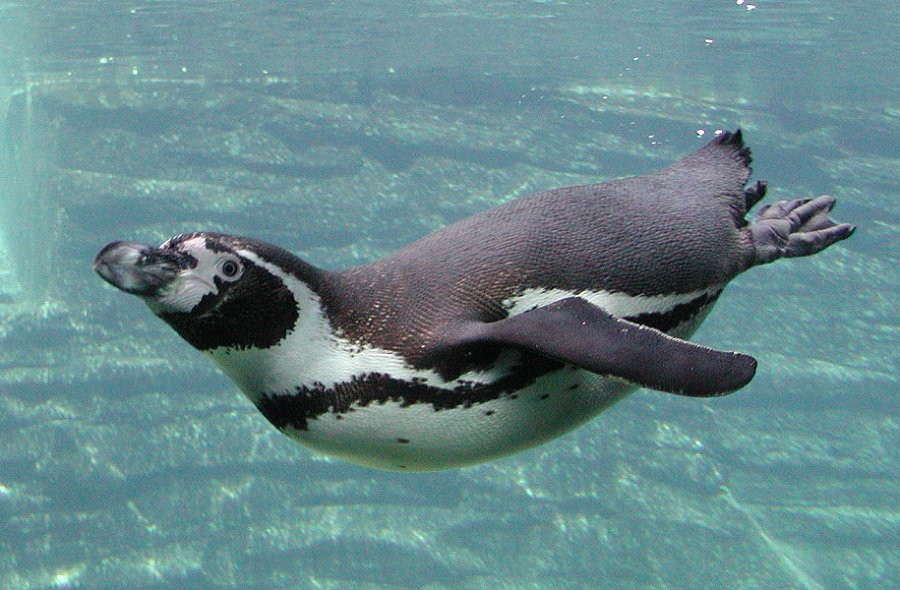
\includegraphics[width=4cm]{images/swim-Ping.jpg}
\caption{A living penguin}
\label{img:pen}
\end{center}
\end{figure}

\subsection{Explanation 2}
It is also said that the word \emph{"penguin"} origianlly was a common name for the also flightless \textbf{great auk} of the northern hemisphere, that went extinct in 1844 (see picture \ref{img:auk}).

\begin{figure}[H]
\begin{center}
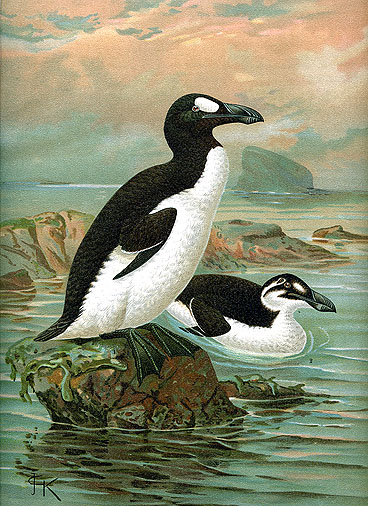
\includegraphics[width=5cm]{images/GreatAuk.jpg}
\caption{Great auks}
\label{img:auk}
\end{center}
\end{figure}

\newpage
\subsection{Explanation 3}
Another theory is that the name stems from the latin word \emph{"penguis"}. It means \emph{"fat"}. For sailors, fat was very important and it could be won from \textbf{penguins} (see picture \ref{img:tux}).

\begin{figure}[H]
\begin{center}

\includegraphics[width=5cm]{images/tux.png}
\caption{Tiny Tux}
\label{img:tux}
\end{center}
\end{figure}
\section{Formulas}
\begin{frame}
\frametitle{Formulas}
\framesubtitle{Use Of Mathematical Formulas}

\begin{exampleblock}{New packages in this section}
\begin{multicols}{2}
\begin{itemize}
\item amsmath 
\item amsthm
\item amssymb
\item mathtools
\end{itemize}
\end{multicols}
\end{exampleblock}

\begin{block}{New commands in this section}
\begin{multicols}{2}
\begin{itemize}
\item \color{nounibaredI}\textbackslash sqrt\color{black}\{\}
\item \color{nounibaredI}\textbackslash frac\color{black}\{\}\{\}
\item \color{nounibaredI}\textbackslash int\color{black}\_X
\item \color{nounibaredI}\textbackslash sum\color{black}\_\{\}
\item \color{nounibaredI}\textbackslash lim\color{black}\_\{\}
\item \color{nounibaredI}\textbackslash prod\color{black}
\item \color{nounibaredI}\textbackslash limits\color{black}\_\{\}
\item \color{nounibaredI}\textbackslash dots\color{black}
\item \color{nounibaredI}\textbackslash cdot\color{black}
\item \color{nounibaredI}\_\color{black}
\item \color{nounibaredI}\^~\color{black}
\end{itemize}
\end{multicols}
\end{block}

\end{frame}

%-------------------------------------------------------------------------------
\begin{frame}
\frametitle{Formulas}
\framesubtitle{\ldots ~A Marvel Of Beauty In \LaTeX !}

\begin{columns}
\begin{column}{.3\textwidth}
{\huge $2 \sqrt{\frac{\pi ^2}{3}\cdot c_{2}}$}
\end{column}

\begin{column}{.7\textwidth}
	$\underbrace{
	\color{unibayellowI}\text{\$}
	\color{black}2
	\color{nounibaredI}\backslash \text{sqrt}
	\color{black}\{
	\color{nounibaredI}\backslash \text{frac}
	\color{black}\{
	\color{nounibaredI}\backslash \text{pi}\color{nounibaredI}
	~\hat{}~\color{black}2\}\{3\color{black}\}
	\color{nounibaredI}\backslash
	\color{nounibaredI}\text{cdot}~
	\color{black} \text{c}
	\color{nounibaredI}\_
	\color{black}2\}
	\color{unibayellowI}\text{\$}
}$
\color{black}

The formula-environment begins and ends with \color{unibayellowI}\$ \color{black} .

\medskip
	$\underbrace{
	\color{nounibaredI}\backslash \text{sqrt}
	\color{black}\{
	\color{nounibaredI}\backslash \text{frac}
	\color{black}\{
	\color{nounibaredI}\backslash \text{pi}\color{nounibaredI}
	~\hat{}~\color{black}2\}\{3\color{black}\}
	\color{nounibaredI}\backslash
	\color{nounibaredI}\text{cdot}~
	\color{black} \text{c}
	\color{nounibaredI}\_
	\color{black}2\}
}$
\color{black}


This whole part is the radical.

\bigskip
$\underbrace{
	\color{nounibaredI}\backslash \text{frac}
	\color{black}\{
	\color{nounibaredI}\backslash \text{pi}\color{nounibaredI}
	~\hat{}~\color{black}2\}\{3\color{black}\}
}$

A fraction has always a numerator and a denominator.
\end{column}
\end{columns}
\end{frame}

%-------------------------------------------------------------------------------

\begin{frame}
\frametitle{Formulas}
\framesubtitle{\ldots ~A Marvel Of Beauty In \LaTeX !}
\begin{columns}
	\begin{column}{.4\textwidth}
		\flushright
		$\int_0^\infty$
	\end{column}
	\begin{column}{.6\textwidth}
		\flushleft
		{\ttfamily\color{unibayellowI}\$\color{nounibaredI}\textbackslash\color{nounibaredI}int\_\color{black}0\color{nounibaredI}\textasciicircum \textbackslash infty\color{unibayellowI}\$}
	\end{column}
\end{columns}
\begin{columns}
	\begin{column}{.4\textwidth}
		\flushright
		$\sum_{i=1}^n$
	\end{column}
	\begin{column}{.6\textwidth}
		\flushleft
		{\ttfamily \color{unibayellowI}\$\color{nounibaredI}\textbackslash
			\color{nounibaredI}sum\_\color{black}\{i=1\}\color{nounibaredI}\textasciicircum
			\color{black}n\color{unibayellowI}\$}
	\end{column}
\end{columns}

\begin{columns}
	\begin{column}{.4\textwidth}
		\flushright
		$\lim_{n \rightarrow \infty}$
	\end{column}
	\begin{column}{.6\textwidth}
		\flushleft
		{\ttfamily \color{unibayellowI}\$\color{nounibaredI}\textbackslash
			\color{nounibaredI}lim\_\color{black}\{n \color{nounibaredI}\textbackslash
			\color{nounibaredI}rightarrow \color{nounibaredI}\textbackslash infty\color{black}\}\color{unibayellowI}\$}
	\end{column}
\end{columns}

\begin{columns}
	\begin{column}{.4\textwidth}
		\flushright
		$\prod\limits_{i=1}^{n+1}i = 1 \cdot 2 \cdot \ldots \cdot n \cdot (n+1)$
	\end{column}
	\begin{column}{.6\textwidth}
		\flushleft
		{\ttfamily \color{unibayellowI}\$%
			\color{nounibaredI}\textbackslash\color{nounibaredI}prod\textbackslash  limits\_\color{black}\{i=1\}\color{nounibaredI}\^{}\color{black}\{n+1\} i = 1 \color{nounibaredI}\textbackslash \color{nounibaredI}cdot \color{black}2 \color{nounibaredI}\textbackslash \color{nounibaredI}cdot \color{nounibaredI}\textbackslash \color{nounibaredI}ldots \color{nounibaredI}\textbackslash\color{nounibaredI}cdot \color{black}n \color{nounibaredI}\textbackslash \color{nounibaredI}cdot \color{black}(n+1)\color{unibayellowI}\$}
	\end{column}
\end{columns}
\bigskip
The American Mathematical Society has a wonderful guide for the {\ttfamily amsmath}-package.\footnote{ftp://ftp.ams.org/pub/tex/doc/amsmath/amsldoc.pdf}
\end{frame}
\section{Tables}

\begin{frame}
\frametitle{Tables}
\framesubtitle{Insertion Of Tables}

\begin{exampleblock}{New packages in this section}
\begin{itemize}
\item longtable
\end{itemize}
\end{exampleblock}

\begin{block}{New commands in this section}
\begin{itemize}
\item \color{unibablueI}\textbackslash begin\color{black}\{tabular\} \dots
~\color{unibablueI}\textbackslash end\color{black}\{tabular\}
\item \color{unibablueI}\textbackslash begin\color{black}\{table\} \dots
~\color{unibablueI}\textbackslash end\color{black}\{table\}
\item \color{unibablueI}\textbackslash begin\color{black}\{longtable\} \dots
~\color{unibablueI}\textbackslash end\color{black}\{longtable\}
\item \color{unibablueI}\textbackslash begin\color{black}\{tabbing\} \dots
~\color{unibablueI}\textbackslash end\color{black}\{tabbing\}
\item \color{nounibaredI}$|$\color{black}
\item \color{nounibaredI}\& \color{black}
\item \color{nounibaredI}\textbackslash hline\color{black}
\item \color{nounibaredI}\textbackslash multicolumn\color{black}\{\}\{\}\{\}
\end{itemize}
\end{block}

\end{frame}

\begin{frame}
\frametitle{Tables}
\framesubtitle{``table'' \& \glqq tabular\grqq}
\textbf{Structure:}\\[2mm]
\color{unibablueI}\begin{ttfamily}\textbackslash begin\color{black}\{table\}\color{nounibagreenI}[position]\color{black}\\
\color{unibablueI}\textbackslash begin\color{black}\{tabular\}\{\textit{Definition of columns}\}\\
\textit{Table content}\\
\color{unibablueI}\textbackslash end\color{black}\{tabular\}\\
\color{nounibaredI}\textbackslash caption\color{black}\{caption\}\\
\color{nounibaredI}\textbackslash label\color{black}\{tab:bsptab1\}\\
\color{unibablueI}\textbackslash end\color{black}\{table\}\\
~\\
\end{ttfamily}

\begin{block}{Reminder: positioning in most \LaTeX -- environments}
\color{nounibagreenI}[h]\color{black}~or \color{nounibagreenI}[H]\color{black}~= At this very position\\
\color{nounibagreenI}[t]\color{black}~= On top of the page\\ 
\color{nounibagreenI}[b]\color{black}~= On bottom of the page\\ 
\color{nounibagreenI}[p]\color{black}~= Positioning on an own page
\end{block}
\end{frame}


\begin{frame}
\frametitle{Tables}
\framesubtitle{Definition Of Columns}
Here you can define how the columns should be aligned
and how the vertical lines should be set:\\[3mm]
\begin{tabbing}[H]p{column width}xxx\=\kill
\textbf{Commands:}\\
l \>= left-justified\\
c \>= centered\\
r \>= right-justified\\
p\{column width\} \>= a left-justified column with defined width\\
\color{nounibaredI}$|$\color{black} \>= sets a vertical line
at this position\\
\end{tabbing}
\end{frame}

\begin{frame}
\frametitle{Tables}
\framesubtitle{View From Inside}
\begin{ttfamily}
\color{nounibaredI}\color{unibablueI}\textbackslash\color{unibablueI}begin\color{black}\color{black}\{tabular\}\{c\color{nounibaredI}|\color{black}p\{40mm\}\color{nounibaredI}|\color{black}lr\color{nounibaredI}|\color{black}c\} \\
\color{nounibaredI}\color{nounibaredI}\textbackslash multicolumn\color{black}\{5\}\{c\}\{E-Sports Championship Franconia\} \color{nounibaredI}\color{nounibaredI}\textbackslash \color{nounibaredI}\textbackslash \color{black} \\
\color{nounibaredI}\color{nounibaredI}\textbackslash hline\color{black} \\
\color{nounibaredI}\color{nounibaredI}\textbackslash hline\color{black} \\
Number \color{nounibaredI}\&  \color{black}Place \color{nounibaredI}\&  \color{black}Player 1 \color{nounibaredI}\&  \color{black}Player 2 \color{nounibaredI}\&  \color{black}Result \color{nounibaredI}\color{nounibaredI}\textbackslash \color{nounibaredI}\textbackslash \color{black} \\
\color{nounibaredI}\color{nounibaredI}\textbackslash hline\color{black} \\
1 \color{nounibaredI}\&  \color{black}Nürnberg \color{nounibaredI}\&  \color{black}Wolf \color{nounibaredI}\&  \color{black}Lamm \color{nounibaredI}\&  \color{black}23:10 \color{nounibaredI}\color{nounibaredI}\textbackslash \color{nounibaredI}\textbackslash \color{black} \\
\color{nounibaredI}\color{nounibaredI}\textbackslash hline\color{black} \\
2 \color{nounibaredI}\&  \color{black}Bamberg \color{nounibaredI}\&  \color{black}Meyer \color{nounibaredI}\&  \color{black}Beyer \color{nounibaredI}\color{nounibaredI}\textbackslash \color{nounibaredI}\textbackslash \color{black} \\
\color{nounibaredI}\color{nounibaredI}\textbackslash hline\color{black} \\
3 \color{nounibaredI}\&  \color{black}Zirndorf \color{nounibaredI}\&  \color{black}Brandst. \color{nounibaredI}\&  \color{black}Brauer \color{nounibaredI}\&  \color{black}21:21\color{nounibaredI}\color{nounibaredI}\textbackslash \color{nounibaredI}\textbackslash \color{black} \\
\color{nounibaredI}\color{nounibaredI}\textbackslash hline\color{black} \\
\color{nounibaredI}\color{unibablueI}\textbackslash\color{unibablueI}end\color{black}\color{black}\{tabular\} \\

\end{ttfamily}
\end{frame}

\begin{frame}
\frametitle{Tables}
\framesubtitle{Table Content}
Here you fill the defined columns with content.\\[3mm]
\begin{tabbing}[H]p{column width}xxx\=\kill
\textbf{Commands:}\\
\color{nounibaredI}\&\color{black} \>= horizontal separation of rows\\
\color{nounibaredI}\textbackslash \textbackslash \color{black} \>=  new line\\
\color{nounibaredI}\textbackslash hline\color{black} \>= sets a horizontal line\\[2mm]
\color{nounibaredI}\textbackslash multicolumn\color{black}\{column number\}\{column alignment\}\{text\}\\[2mm]
\>= Combines as many columns as you like.\\
\end{tabbing}
\end{frame}

\begin{frame}[t]

\frametitle{Tables}
\framesubtitle{Example Tabular}
\begin{footnotesize}
\begin{ttfamily}
\color{nounibaredI}\color{unibablueI}\textbackslash\color{unibablueI}begin\color{black}\color{black}\{tabular\}\{c\color{nounibaredI}|\color{black}p\{40mm\}\color{nounibaredI}|\color{black}lr\color{nounibaredI}|\color{black}c\} \\
\color{nounibaredI}\color{nounibaredI}\textbackslash multicolumn\color{black}\{5\}\{c\}\{E-Sports Championship Franconia\} \color{nounibaredI}\color{nounibaredI}\textbackslash \color{nounibaredI}\textbackslash \color{black} \\
\color{nounibaredI}\color{nounibaredI}\textbackslash hline\color{black} \\
\color{nounibaredI}\color{nounibaredI}\textbackslash hline\color{black} \\
Number \color{nounibaredI}\&  \color{black}Place \color{nounibaredI}\&  \color{black}Player 1 \color{nounibaredI}\&  \color{black}Player 2 \color{nounibaredI}\&  \color{black}Result \color{nounibaredI}\color{nounibaredI}\textbackslash \color{nounibaredI}\textbackslash \color{black} \\
\color{nounibaredI}\color{nounibaredI}\textbackslash hline\color{black} \\
1 \color{nounibaredI}\&  \color{black}Nürnberg \color{nounibaredI}\&  \color{black}Wolf \color{nounibaredI}\&  \color{black}Lamm \color{nounibaredI}\&  \color{black}23:10 \color{nounibaredI}\color{nounibaredI}\textbackslash \color{nounibaredI}\textbackslash \color{black} \\
\color{nounibaredI}\color{nounibaredI}\textbackslash hline\color{black} \\
2 \color{nounibaredI}\&  \color{black}Bamberg \color{nounibaredI}\&  \color{black}Meyer \color{nounibaredI}\&  \color{black}Beyer \color{nounibaredI}\color{nounibaredI}\textbackslash \color{nounibaredI}\textbackslash \color{black} \\
\color{nounibaredI}\color{nounibaredI}\textbackslash hline\color{black} \\
3 \color{nounibaredI}\&  \color{black}Zirndorf \color{nounibaredI}\&  \color{black}Brandst. \color{nounibaredI}\&  \color{black}Brauer \color{nounibaredI}\&  \color{black}21:21\color{nounibaredI}\color{nounibaredI}\textbackslash \color{nounibaredI}\textbackslash \color{black} \\
\color{nounibaredI}\color{nounibaredI}\textbackslash hline\color{black} \\
\color{nounibaredI}\color{unibablueI}\textbackslash\color{unibablueI}end\color{black}\color{black}\{tabular\} \\

\end{ttfamily}
\end{footnotesize}

\begin{tabular}{c|p{40mm}|lr|c}
\multicolumn{5}{c}{E-Sports Championship Franconia}
 \\
\hline
\hline
Number & Place & Player 1 & Player 2 & Result \\
\hline
1 & N\"urnberg & Wolf & Lamm & 23:10 \\
\hline
2 & Bamberg & Meyer & Beyer & \\
\hline
3 & Zirndorf & Brandst. & Brauer & 21:21 \\
\hline
\end{tabular}
\end{frame}

\begin{frame}{Tables}
\framesubtitle{Longtable -- Table With Line Break}
\bigskip
„tabular“ shows the table on one page. If it does not fit on the page, the remainder is cut off.\\
For tables longer than one page, a table is needed that performs a division of the table.\\
\textbf{Solution: {\ttfamily longtable}}\\
{\ttfamily longtable} allows a line break in the table. Moreover, {\ttfamily longtable} is an environment, so the  {\ttfamily table}-environment is not needed anymore!\\[3mm]

\begin{ttfamily}
\color{unibablueI}\textbackslash begin\color{black}\{longtable\}\{\textit{definition of columns}\}\\
\textit{table content}\\
\color{nounibaredI}\textbackslash caption\color{black}\{caption\}\\
\color{nounibaredI}\textbackslash label\color{black}\{tab:bsptab2\}\\
\color{unibablueI}\textbackslash end\color{black}\{longtable\}
\end{ttfamily}
\end{frame}


\begin{frame}
\frametitle{Indentations With „tabbing“}
\begin{block}{Control}
\begin{itemize}
\item[\begin{ttfamily}\color{nounibaredI}\textbackslash =\end{ttfamily}]\color{black}set a tab position 
\item[\begin{ttfamily}\color{nounibaredI}\textbackslash $>$\end{ttfamily}]select a tab position
\end{itemize}
\end{block}

\begin{columns}
\begin{column}{.5\textwidth}
\begin{ttfamily}{\scriptsize
\color{nounibaredI}\color{nounibaredI}\textbackslash documentclass\color{black}\{article\} \\
\color{nounibaredI}\color{unibablueI}\textbackslash\color{unibablueI}begin\color{black}\color{black}\{document\} \\
\color{nounibaredI}\color{unibablueI}\textbackslash\color{unibablueI}begin\color{black}\color{black}\{tabbing\} \\
Employ\color{nounibaredI}\color{nounibaredI}\textbackslash \color{black}=ee:\color{nounibaredI}\color{nounibaredI}\textbackslash \color{nounibaredI}\textbackslash \color{black} \\
A  \color{nounibaredI}\color{nounibaredI}\textbackslash \color{black}> Daniel\color{nounibaredI}\color{nounibaredI}\textbackslash \color{nounibaredI}\textbackslash \color{black} \\
B  \color{nounibaredI}\color{nounibaredI}\textbackslash \color{black}> Martin\color{nounibaredI}\color{nounibaredI}\textbackslash \color{nounibaredI}\textbackslash \color{black} \\
C  \color{nounibaredI}\color{nounibaredI}\textbackslash \color{black}> Linus\color{nounibaredI}\color{nounibaredI}\textbackslash \color{nounibaredI}\textbackslash \color{black} \\
xxx\color{nounibaredI}\color{nounibaredI}\textbackslash \color{black}=xxx\color{nounibaredI}\color{nounibaredI}\textbackslash \color{black}=xxxxxxx\color{nounibaredI}\color{nounibaredI}\textbackslash kill\color{black} \\
\color{nounibaredI}\color{nounibaredI}\textbackslash \color{black}> Committees\color{nounibaredI}\color{nounibaredI}\textbackslash \color{nounibaredI}\textbackslash \color{black} \\
\color{nounibaredI}\color{nounibaredI}\textbackslash \color{black}>\color{nounibaredI}\color{nounibaredI}\textbackslash \color{black}> Tests\color{nounibaredI}\color{nounibaredI}\textbackslash \color{nounibaredI}\textbackslash \color{black} \\
\color{nounibaredI}\color{nounibaredI}\textbackslash \color{black}>\color{nounibaredI}\color{nounibaredI}\textbackslash \color{black}> Mails\color{nounibaredI}\color{nounibaredI}\textbackslash \color{nounibaredI}\textbackslash \color{black} \\
\color{nounibaredI}\color{unibablueI}\textbackslash\color{unibablueI}end\color{black}\color{black}\{tabbing\} \\
\color{nounibaredI}\color{unibablueI}\textbackslash\color{unibablueI}end\color{black}\color{black}\{document\} \\
}
\end{ttfamily}
\end{column}
\begin{column}{.5\textwidth}
\begin{tabbing}
Employ\=ee:\\
A  \> Daniel\\
B  \> Martin\\
C  \> Linus\\
xxx\=xxx\=xxxxxxx\kill
\> Committees\\
\>\> Tests\\
\>\> Mails\\
\end{tabbing}
\end{column}
\end{columns}

If you use the command \begin{ttfamily}\color{nounibaredI}\textbackslash kill\color{black}\end{ttfamily}, the rest of the line is not shown. In this way you can do the formatting without showing the respective text.
\end{frame}

\section{Enumerations}
\begin{frame}
\frametitle{Enumerations}

\begin{block}{New commands in this section}
\begin{itemize}
\item \color{unibablueI}\textbackslash begin\color{black}\{itemize\} \ldots \color{unibablueI}\textbackslash end\color{black}\{itemize\} 
\item \color{unibablueI}\textbackslash begin\color{black}\{enumerate\} \ldots \color{unibablueI}\textbackslash end\color{black}\{enumerate\} 
\item \color{nounibaredI}\textbackslash item\color{black}
\end{itemize}
\end{block}
\end{frame}

\begin{frame}
\frametitle{Enumerations}
\framesubtitle{Bulleted List}

\begin{columns}
\begin{column}{.5\textwidth}
\begin{ttfamily}
\color{nounibaredI}\color{nounibaredI}\textbackslash documentclass\color{black}\{article\} \\
\color{nounibaredI}\color{unibablueI}\textbackslash\color{unibablueI}begin\color{black}\color{black}\{document\} \\
\color{nounibaredI}\color{unibablueI}\textbackslash\color{unibablueI}begin\color{black}\color{black}\{itemize\} \\
\color{nounibaredI}\color{nounibaredI}\textbackslash item \color{black} first bullet item \\
\color{nounibaredI}\color{nounibaredI}\textbackslash item \color{black} second bullet item \\
\color{nounibaredI}\color{nounibaredI}\textbackslash item \color{black} third bullet item \\
\color{nounibaredI}\color{nounibaredI}\textbackslash item \color{black} last bullet item \\
\color{nounibaredI}\color{unibablueI}\textbackslash\color{unibablueI}end\color{black}\color{black}\{itemize\} \\
\color{nounibaredI}\color{unibablueI}\textbackslash\color{unibablueI}end\color{black}\color{black}\{document\} \\
\end{ttfamily}
\end{column}
\begin{column}{.5\textwidth}
\begin{itemize}
\item first bullet item
\item second bullet item
\item third bullet item
\item last  bullet item
\end{itemize}
\end{column}
\end{columns}
\bigskip

The particular bullet items are indicated in the „itemize“-environment with the command \begin{ttfamily}\color{nounibaredI}\textbackslash item\color{black}\end{ttfamily}.
\end{frame}

\begin{frame}
\frametitle{Enumerations}
\framesubtitle{Interlacing}

\begin{columns}
\begin{column}{.5\textwidth}
\begin{ttfamily}
\color{nounibaredI}\color{nounibaredI}\textbackslash documentclass\color{black}\{article\} \\
\color{nounibaredI}\color{unibablueI}\textbackslash\color{unibablueI}begin\color{black}\color{black}\{document\} \\
\color{nounibaredI}\color{unibablueI}\textbackslash\color{unibablueI}begin\color{black}\color{black}\{itemize\} \\
\color{nounibaredI}\color{nounibaredI}\textbackslash item \color{black} first bullet item \\
\color{nounibaredI}\color{nounibaredI}\textbackslash item \color{black} second bullet item \\
\color{nounibaredI}\color{unibablueI}\textbackslash\color{unibablueI}begin\color{black}\color{black}\{itemize\} \\
\color{nounibaredI}\color{nounibaredI}\textbackslash item \color{black} first subitem \\
\color{nounibaredI}\color{nounibaredI}\textbackslash item \color{black} second subitem \\
\color{nounibaredI}\color{unibablueI}\textbackslash\color{unibablueI}end\color{black}\color{black}\{itemize\} \\
\color{nounibaredI}\color{nounibaredI}\textbackslash item \color{black} third bullet item \\
\color{nounibaredI}\color{nounibaredI}\textbackslash item \color{black} last bullet item \\
\color{nounibaredI}\color{unibablueI}\textbackslash\color{unibablueI}end\color{black}\color{black}\{itemize\} \\
\color{nounibaredI}\color{unibablueI}\textbackslash\color{unibablueI}end\color{black}\color{black}\{document\} \\
\end{ttfamily}
\end{column}
\begin{column}{.5\textwidth}
\begin{itemize}
\item first bullet item
\item second bullet item
\begin{itemize}
\item first subitem
\item second subitem
\end{itemize}
\item third bullet item
\item last bullet item
\end{itemize}
\end{column}
\end{columns}
\bigskip
In this way, subitems can be interlaced in maximal four layers.
\end{frame}


\begin{frame}
\frametitle{Enumerations}
\framesubtitle{Numerations}

\begin{columns}
\begin{column}{.5\textwidth}
\begin{ttfamily}
\color{nounibaredI}\color{nounibaredI}\textbackslash documentclass\color{black}\{article\} \\
\color{nounibaredI}\color{unibablueI}\textbackslash\color{unibablueI}begin\color{black}\color{black}\{document\} \\
\color{nounibaredI}\color{unibablueI}\textbackslash\color{unibablueI}begin\color{black}\color{black}\{enumerate\} \\
\color{nounibaredI}\color{nounibaredI}\textbackslash item \color{black} first bullet item \\
\color{nounibaredI}\color{unibablueI}\textbackslash\color{unibablueI}begin\color{black}\color{black}\{enumerate\} \\
\color{nounibaredI}\color{nounibaredI}\textbackslash item \color{black} first subitem \\
\color{nounibaredI}\color{nounibaredI}\textbackslash item \color{black} second subitem \\
\color{nounibaredI}\color{unibablueI}\textbackslash\color{unibablueI}end\color{black}\color{black}\{enumerate\} \\
\color{nounibaredI}\color{nounibaredI}\textbackslash item \color{black} second bullet item \\
\color{nounibaredI}\color{nounibaredI}\textbackslash item \color{black} and so forth \\
\color{nounibaredI}\color{unibablueI}\textbackslash\color{unibablueI}end\color{black}\color{black}\{enumerate\} \\
\color{nounibaredI}\color{unibablueI}\textbackslash\color{unibablueI}end\color{black}\color{black}\{document\} \\
\end{ttfamily}
\end{column}
\begin{column}{.5\textwidth}
\begin{enumerate}
\item first bullet item
\begin{enumerate}
\item first subitem
\item second subitem
\end{enumerate}
\item second bullet item
\item and so forth
\end{enumerate}
\end{column}
\end{columns}
\bigskip
Again, the particular bullet items are indicated with the command \begin{ttfamily}\color{nounibaredI}\textbackslash item\color{black}\end{ttfamily}. 
Again there are four layers for interlacing.
\end{frame}

\begin{frame}
\frametitle{Mixed Enumerations?}
\framesubtitle{Of Course!}

\begin{columns}
\begin{column}{.5\textwidth}
\begin{ttfamily}
\color{nounibaredI}\color{unibablueI}\textbackslash\color{unibablueI}begin\color{black}\color{black}\{enumerate\} \\
\color{nounibaredI}\color{nounibaredI}\textbackslash item \color{black} first bullet item \\
\color{nounibaredI}\color{nounibaredI}\textbackslash item \color{black} \color{nounibaredI}\color{unibablueI}\textbackslash\color{unibablueI}begin\color{black}\color{black}\{itemize\} \\
\color{nounibaredI}\color{nounibaredI}\textbackslash item \color{black} first subitem \\
\color{nounibaredI}\color{nounibaredI}\textbackslash item \color{black} second subitem \\
\color{nounibaredI}\color{unibablueI}\textbackslash\color{unibablueI}end\color{black}\color{black}\{itemize\} \\
\color{nounibaredI}\color{nounibaredI}\textbackslash item \color{black} third bullet item \\
\color{nounibaredI}\color{unibablueI}\textbackslash\color{unibablueI}begin\color{black}\color{black}\{enumerate\} \\
\color{nounibaredI}\color{nounibaredI}\textbackslash item \color{black} I matter, too! \\
\color{nounibaredI}\color{unibablueI}\textbackslash\color{unibablueI}end\color{black}\color{black}\{enumerate\} \\
\color{nounibaredI}\color{nounibaredI}\textbackslash item \color{black} and so forth \\
\color{nounibaredI}\color{unibablueI}\textbackslash\color{unibablueI}end\color{black}\color{black}\{enumerate\} \\
\end{ttfamily}
\end{column}
\begin{column}{.5\textwidth}
\begin{enumerate}
\item first bullet item
\item \begin{itemize}
\item first subitem
\item second subitem
\end{itemize}
\item third bullet item
\begin{enumerate}
\item I matter, too!
\end{enumerate}
\item and so forth
\end{enumerate}
\end{column}
\end{columns}
\bigskip
You can customize the symblos with \color{nounibaredI}\textbackslash item\color{nounibagreenI}[]\color{black}. 
\end{frame}
\section{$\mathcal{T}4$} 
\begin{frame}
\frametitle{Task 4}
\framesubtitle{Recreate Task4.pdf in \LaTeX !} 

\begin{block}{Task 4}
\begin{itemize}
  \item Don't forget the \color{nounibaredII}\textbackslash \textbackslash  \color{black}~ at the end of a table row!%
  \item Pay attention to the interlacing of the \color{nounibaredII}\textbackslash item\color{black}s%
  \item It can be useful to indent the code for a better overview%
\end{itemize}
\end{block}
\end{frame}
\section{Distributed Work}
\begin{frame}
\frametitle{Build A Stout Document}
\framesubtitle{\ldots And Experience The Real Congeniality Of \LaTeX !}
\begin{block}{New commands in this section}
\begin{itemize}
  \item \color{nounibaredI}\textbackslash input\color{black}\{\}
  \item \color{nounibaredI}\textbackslash tableofcontents\color{black}
  \item \color{nounibaredI}\textbackslash listoffigures\color{black}
  \item \color{nounibaredI}\textbackslash listoftables\color{black}
  \item \color{nounibaredI}\textbackslash vspace\color{black}\{\}
  \item \color{nounibaredI}\textbackslash today\color{black}
\item \color{unibablueI}\textbackslash begin\color{black}\{titlepage\} \ldots \color{unibablueI}\textbackslash end\color{black}\{titlepage\} 
\end{itemize}
\end{block}
\end{frame}

\begin{frame}
\frametitle{Building A Bigger Document}

\begin{columns}
\begin{column}{.5\textwidth}
\footnotesize
\begin{figure}[t]
\begin{tikzpicture}[dirtree]
\node {main.tex} 
        child {node {command.tex}}
        child {node {titlepage.tex}}
        child {node {introduction.tex}}
        child {node {task1.tex}}
        child {node {task2.tex}}
        child {node {task3.tex}}
        child {node {conclusion.tex}};
\end{tikzpicture}
\end{figure}
\end{column}
\begin{column}{.5\textwidth}
All other files are combined to one document in the file main.tex. 
For this, you have to adjust the other files.
\end{column}
\end{columns}
\end{frame}

\begin{frame}
\frametitle{\ldots ~let's do it!}
You have to delete \textbf{everything} (including) before and after \color{unibablueI}\textbackslash begin\color{black}- 
and\color{unibablueI}~\textbackslash end\color{black}\{document\}:\\[5mm]
\begin{columns}
\begin{column}{.47\textwidth}
\sout{\color{nounibaredI}\color{nounibaredI}\textbackslash documentclass\color{black}\color{nounibagreenI}[pdftex]\color{black}\{article\} \\
\color{nounibaredI}\textbackslash usepackage\color{black}\{babel\}\\
\color{nounibaredI}\color{unibablueI}\textbackslash\color{unibablueI}begin\color{black}\color{black}\{document\} }\\
This document can now be included in LaTeX using the command \color{nounibaredI}\color{nounibaredI}\textbackslash input\color{nounibaredI}\color{black}\{file name\}.\\
\sout{\color{nounibaredI}\color{unibablueI}\textbackslash\color{unibablueI}end\color{black}\color{black}\{document\} }
\end{column}
\begin{column}{.47\textwidth}
With the command \color{nounibaredI}\textbackslash input\color{black}\{path/to/file\} you can afterwards
 include this into another {\ttfamily .tex}-file. 

\end{column}
\end{columns}
\end{frame}

\begin{frame}
\frametitle{Distributed Work}
\framesubtitle{\ldots Stay On Top Of Things}
\begin{columns}{2}
\begin{column}{.6\textwidth}
\image{\textwidth}{image/outline.png}{Texmaker lists the {\ttfamily\color{nounibaredI}\textbackslash input}\color{black}s}{img:outline}
\end{column}
\begin{column}{.3\textwidth}
\begin{alertblock}{Attention:}
The path declaration is always relative to the main file!
\end{alertblock}
\end{column}
\end{columns}

\end{frame}


\begin{frame}[t]
\frametitle{Excursus: Title Page}
\begin{columns}
\begin{column}{0.5\textwidth}
\begin{titlepage}
\begin{center}
\vspace*{20mm}{\Huge \LaTeX}\\
\vspace{5mm} {\LARGE A Short Introduction}\\
\vspace{12mm} {\LARGE University of\\ Bamberg}\\
\vspace{24mm} {Fachschaft WIAI\\ \href{mailto: fachschaft.wiai@uni-bamberg.de}{fachschaft.wiai@uni-bamberg.de}}\\
\end{center}
\end{titlepage}
\end{column}
\begin{column}{0.5\textwidth}
\color{nounibaredI}\color{unibablueI}\textbackslash\color{unibablueI}begin\color{black}\color{black}\{titlepage\} \\\color{black}
\color{nounibaredI}\color{unibablueI}\textbackslash\color{unibablueI}begin\color{black}\color{black}\{center\} \\
\color{nounibaredI}\color{nounibaredI}\textbackslash Huge\color{black} \color{nounibaredI}\color{nounibaredI}\textbackslash LaTeX\color{nounibaredI}\textbackslash \color{nounibaredI}\textbackslash \color{black} \\
\color{nounibaredI}\color{nounibaredI}\textbackslash vspace\color{black}\{5mm\} \color{nounibaredI}\color{nounibaredI}\textbackslash LARGE \color{black} A Short Introduction\color{nounibaredI}\color{nounibaredI}\textbackslash \color{nounibaredI}\textbackslash \color{black} \\
\color{nounibaredI}\color{nounibaredI}\textbackslash vspace\color{black}\{12mm\} \color{nounibaredI}\color{nounibaredI}\textbackslash Large \color{black} University of Bamberg\color{nounibaredI}\color{nounibaredI}\textbackslash \color{nounibaredI}\textbackslash \color{black}\color{nounibagreenI}[5mm]\color{black} \\
\color{nounibaredI}\color{nounibaredI}\textbackslash large\color{black} \color{nounibaredI}\color{nounibaredI}\textbackslash today\color{nounibaredI}\textbackslash \color{nounibaredI}\textbackslash \color{black} \\
Fachschaft WIAI\color{nounibaredI}\color{nounibaredI}\textbackslash normalsize\color{black} \color{nounibaredI}\color{nounibaredI}\textbackslash \color{nounibaredI}\textbackslash \color{black} \\
\color{nounibaredI}\color{unibablueI}\textbackslash\color{unibablueI}end\color{black}\color{black}\{center\} \\
\color{nounibaredI}\color{unibablueI}\textbackslash\color{unibablueI}end\color{black}\color{black}\{titlepage\} \\\color{black}
\end{column}
\end{columns}
\end{frame}


\begin{frame}
\frametitle{Distributed Work}
\framesubtitle{Commands For Page Numbering}
\begin{block}{Page Numbering}
\begin{itemize}
\item \color{nounibaredI}\textbackslash thispagestyle\color{black}\{empty\} -- No page numbering
\item \color{nounibaredI}\textbackslash setcounter\color{black}\{page\}\{1\} -- Sets a defined value as page number
\item \color{nounibaredI}\textbackslash pagenumbering\color{black}\{Roman$\mid$roman$\mid$arabic$\mid$Alph$\mid$alph\} -- Defines the page numbering
\item \color{nounibaredI}\textbackslash  newpage \color{black}-- Creates a new page
\end{itemize}
\end{block}
\end{frame}

\section{$\mathcal{T}5$}

\begin{frame}
\frametitle{Task 5}
\framesubtitle{Recreate one of the two layouts for task 5 in \LaTeX !}

\begin{block}{Task 5}
\begin{itemize}
\item Build a title page!%
\item Use task $\mathcal{T}2$ to $\mathcal{T}4$ as content.%
\item Pay attention to correct page numbering!%
\item Decide for one of the two layouts from the VC-course.%
\end{itemize}
\end{block}
\end{frame}
\section{BibTeX}
\begin{frame}
\frametitle{BibTeX}
\framesubtitle{Add On For \LaTeX}
\begin{exampleblock}{New packages in this section}
\begin{itemize}
\item natbib
\end{itemize}
\end{exampleblock}

\begin{block}{New commands in this section}
\begin{itemize}
%\item \color{nounibaredI}\textbackslash renewcommand\color{black}\{\color{nounibaredI}\textbackslash refname\color{black}\}\{...\}
\item \color{nounibaredI}\textbackslash cite\color{black}\{Author2014\}
\item \color{nounibaredI}\textbackslash bibliographystyle\color{black}\{alpha$\mid$abbrv$\mid$natdin$\mid$apa$\mid$etc.\}
\item \color{nounibaredI}\textbackslash bibliography\color{black}\{literature.bib\}
%\item \color{nounibaredI}\textbackslash addcontentsline\color{black}\{toc\}\{section\}\{\color{nounibaredI}\textbackslash refname\color{black}\}
\end{itemize}
\end{block}
\end{frame}

\begin{frame}
\frametitle{BibTeX And \LaTeX ~In Combiantion}
\textbf{Advantages:}
\begin{itemize}
\item List of literature is saved in an extra \texttt{.bib}-file, independent from the document.
\item Save data in BibTeX -format. Here you can distinguish the type of source, e.g. with \color{nounibaredI}$@$book\color{black},~\color{nounibaredI}$@$article\color{black}~usw.
\item Wide range of quoting styles
\item \textbf{Automated creation of the list of literature (LOL), corresponding to the style}
\item Inclusion of an entry in the LOL only if the source is mentioned in the text
\end{itemize}
\textbf{Disadvantages:}
\begin{itemize}
\item The creation of a LOL with special demands is potentially complicated
\end{itemize}
\end{frame}

\begin{frame}
\frametitle{BibTeX And \LaTeX ~In Combination}
\framesubtitle{BibTeX -files}
\begin{columns}
\begin{column}{0.52\textwidth}
\textbf{Example entry:}\\[1em]

\color{nounibaredI}$@$book\color{black}\{Culik93,\\
\color{nounibaredI}title\color{black} = \{Die Welt der Pinguine\},\\
\color{nounibaredI}author\color{black} = \{B.M. Culik and R. P. Wilson\},\\
\color{nounibaredI}publisher\color{black} = \{\{BLV\}M"unchen\},\\
\color{nounibaredI}year\color{black} = \{1993\}\\
\}
\end{column}
\begin{column}{0.55\textwidth}
\textbf{Explanation of entry:}
\begin{itemize}
\item \color{nounibaredI}$@$book\color{black}~- Specification of the type of source, here a book
\item Culik93 - Definition of an unique reference key
\item \color{nounibaredI}author\color{black}~- Author of the book
\item \color{nounibaredI}title\color{black}~- Title of the book
\item \color{nounibaredI}publisher\color{black}~- Publisher
\item \color{nounibaredI}year\color{black}~- Year of publication
\end{itemize}
\end{column}
\end{columns}
\begin{alertblock}{Attention: Consider order for compiling!}
(1) pdflatex (2) bibtex (3) pdflatex (4) pdflatex
\end{alertblock}
\end{frame}

\begin{frame}
\frametitle{BibTeX And \LaTeX ~In Combination}
\framesubtitle{Overview Over Commands}
\begin{itemize}

\item \color{nounibaredI}\textbackslash cite\color{black}\{Culik93\} \hfill Cite a BibTeX entry\\

\item \color{nounibaredI}\textbackslash bibliographystyle\color{black}\{alphadin\} \hfill Select the LOL style \glqq \texttt{alphadin}\grqq\\

\item \color{nounibaredI}\textbackslash bibliography\color{black}\{bibliography.bib\} \hfill Sepcify the  BibTeX -file\\

\item \color{nounibaredI}\textbackslash usepackage\color{black}\{natbib\} \hfill Necessary for quotation style \texttt{natdin}\\
%\item \color{nounibaredI}\textbackslash renewcommand\color{black}\{\color{nounibaredI}\textbackslash refname\color{black}\}\newline \{Literaturverzeichnis\} \hfill Anpassung des Namens von Standard Literatur auf Literaturverzeichnis

%\item \color{nounibaredI}\textbackslash addcontentsline\color{black}\{toc\}\{section\}\newline \{\color{nounibaredI}\textbackslash refname\color{black}\} \hfill Aufnahme des LVZ ins Inhaltsverzeichnis

\end{itemize}


\end{frame}


\begin{frame}
\frametitle{BibTeX And \LaTeX ~In Combination}
\framesubtitle{Examples For Styles}
\image{\textwidth}{image/alpha.png}{Alpha Quotation Style}{img:alpha}
\end{frame}


\begin{frame}
\frametitle{BibTeX And \LaTeX ~In Combination}
\framesubtitle{Examples For Styles cont'd}
\image{\textwidth}{image/IEEEtran.png}{IEEEtran Quotation Style}{img:ieeetran}
\end{frame}

\begin{frame}
\frametitle{BibTeX And \LaTeX ~In Combination}
\framesubtitle{Examples For Styles cont'd}
\image{\textwidth}{image/natdin.png}{Natdin Quotation Style}{img:natdin}
\end{frame}


\begin{frame}
\frametitle{BibTeX And \LaTeX ~In Combination}
\framesubtitle{Examples For Styles cont'd}
\image{\textwidth}{image/apa.png}{Apa Quotation Style}{img:apa}
\end{frame}
%\input{content/beamerclass}



%%%%%%%%%%%%%%%%%%%%%%%%%%%%%%%%%%%%%%%%%
%%%%%%%%%% References          %%%%%%%%%%
%%%%%%%%%%%%%%%%%%%%%%%%%%%%%%%%%%%%%%%%%
%\section*{}
%\begin{frame}[allowframebreaks]{References}
%\def\newblock{\hskip .11em plus .33em minus .07em}
%\scriptsize
%\bibliographystyle{IEEEtran}
%\bibliography{literature/bib}
%\normalsize
%\end{frame}




%% Last frame
\frame{
  \vspace{2cm}
  {\huge Questions ?}

  \vspace{20mm}
  \nocite*
  \vspace{0mm}
  
  \begin{flushright}
  
  Fachschaft WIAI
  
    \structure{\footnotesize{\href{mailto:fachschaft.wiai@uni-bamberg.de}{fachschaft.wiai@uni-bamberg.de}}}
  
  \end{flushright}
  
}


\end{document}
